\startdocument

\section{Cosmology}
\label{SecCO}

The dynamics of our universe is described by Einstein equations in the presence of matter. The Friedmann-Lemaitre-Robertson-Walker (FLRW) metric describing the evolution of the Universe  is based upon the assumption of homogeneity and isotropy, which is approximately true on large scales. These assumptions  determine the metric up to an arbitrary function of time, $a(t)$, the scale factor, which measures the time evolution of the Universe, and a discrete parameter $k = -1,0,1$, which determines the 3-dimensional curvature of the Universe, namely whether it is respectively open, flat or closed.

Small deviations from homogeneity at early epochs played a very important role in the dynamical history of our universe. Small initial density perturbations grew via gravitational instability into the structures that we observe today in the universe. The temperature anisotropies observed in the Cosmic Microwave Background (CMB) are believed to have originated from quantum fluctuations generated during an inflationary stage in the early universe, which we review in Sec. \ref{sec:infla}. In this section we review the main features of the homogeneous and isotropic cosmology necessary for the subsequent sections. For dedicated accounts of the standard $\Lambda$CDM cosmology and the growth of cosmic structure, we also refer the reader to e.g. \cite{Dodelson:2003ft, Weinberg:2008zzc, Mukhanov:2005sc, Baumann:2022mni}. More technical summaries of recent progress and challenges can be found in  \cite{Chou:2022luk, Green:2022hhj, Flauger:2022hie}.
\bigskip

The FLRW metric can be written as:
\be\label{eq:FLRW}
\setlength\fboxsep{0.25cm}
\setlength\fboxrule{0.4pt}
\boxed{
ds^2 = -dt^2 + a(t) \left[dr^2 + f^2_k(r) \left(d\theta^2 +\sin^2{\theta}\,d\phi^2\right) \right] \,,
}
\ee
where
\begin{equation*}
f_k(r) =  \left\{
\begin{array}{rl}
\sin r  & \text{if }\,\, k = +1 ,\\
r & \text{if }\,\, k = 0,\\
\sinh r & \text{if } \,\, k =-1.
\end{array} \right.
\end{equation*}
The dynamics associated with the scale factor $a(t)$ is determined by Einstein's equations:
\be\label{eq:Einstein4D}
\setlength\fboxsep{0.25cm}
\setlength\fboxrule{0.4pt}
\boxed{
G_{\mu\nu} \equiv R_{\mu\nu} -\frac{1}{2} g_{\mu\nu} R = 8\pi\, G_4 \, T_{\mu\nu}\,,
}
\ee
 provided the matter content encoded in the energy-momentum tensor $T_{\mu\nu}$  is specified. Let us consider an ideal perfect fluid as the source of
the energy momentum tensor. In this case we have:
\be\label{eq:EMT4D}
 T^\mu_{\,\,\nu} = {\rm diag}\left(-\rho, p, p, p\right)\,,
 \ee
 where  $\rho$ and  $p$ are the {\em energy density} and {\em pressure} of the fluid, respectively.

Einstein's equations for the metric \eqref{eq:FLRW} and energy-momentum tensor \eqref{eq:EMT4D} give the two independent equations:
\bea
H^2 &=& \frac{8\pi G_4}{3} \rho - \frac{k}{a^2} \,, \label{eq:Fried4DH} \\
\frac{\ddot a}{a} &=& -\frac{4\pi G_4}{3} \left(\rho + 3 \,p\right) \label{eq:Fried4Da}\,,
\eea
 where $H$ is the Hubble parameter (function), defined as
 \be\label{eq:Hdef}
 \setlength\fboxsep{0.25cm}
\setlength\fboxrule{0.4pt}
\boxed{
 H \equiv \frac{\dot a}{a}\,.
 }
 \ee
 The energy momentum tensor is conserved by virtue of the Bianchi identities, $\nabla_\mu T^{\mu\nu} =0$, leading to the continuity equation
 \be\label{eq:EMconsFLRW}
 \setlength\fboxsep{0.25cm}
\setlength\fboxrule{0.4pt}
\boxed{
 \dot\rho + 3H (\rho+p) =0 \,,
 }
 \ee
 which can be derived also from  Einstein's equations above, \eqref{eq:Fried4DH}, \eqref{eq:Fried4Da}. Notice already that eq. \eqref{eq:Fried4Da} implies that in order to have {\em accelerated expansion}, that is $\ddot a>0$, the energy density and pressure must be such that
 \be
 \setlength\fboxsep{0.25cm}
\setlength\fboxrule{0.4pt}
\boxed{
\label{eq:rho3p}
 (\rho+3p) <0\,.
}
\ee

 One can write eq.~\eqref{eq:Fried4DH} in the form
 \be
\label{eq:Omega4D}
 \Omega(t) -1 = \frac{k}{(aH)^2}\,,
 \ee
where we defined the dimensionless density parameter
\be
\setlength\fboxsep{0.25cm}
\setlength\fboxrule{0.4pt}
\boxed{
\label{eq:Omegadef}
\Omega(t) \equiv \frac{\rho(t)}{\rho_c(t)} \,, \qquad \rho_c(t) \equiv \frac{3H^2(t)}{8\pi G_4}\,,}
\ee
with $\rho_c$ the critical density. From here we can see that the matter distribution determines the spatial geometry of our universe:  
  \begin{subequations}\label{eq:OmegaGeo}
\begin{empheq}[box=\widefbox]{align}
 &\Omega >1 \quad {\rm or } \quad  \rho>\rho_c \quad  \Rightarrow \,\,\, k = +1\,, \nonumber \\
 &\Omega =1 \quad {\rm or } \quad \rho=\rho_c \quad   \Rightarrow \,\,\, k = 0\,, \nonumber \\
 & \Omega <1 \quad {\rm or } \quad \rho<\rho_c \quad  \Rightarrow \,\,\, k = -1\,.
 \end{empheq}
\end{subequations}



Observations indicate that the current universe is very close to a spatially flat geometry \cite{Planck:2018vyg}. This is actually a natural result from inflation in the early universe (see below). Hence, in this section we consider a flat universe ($k =0$, $\Omega \simeq 1$). But we will keep an open mind regarding the spatial curvature when we discuss string constructions.

\subsection{Evolution of the Universe Filled with a Perfect Fluid}

Let us now consider the evolution of the universe filled with a barotropic perfect fluid with an equation of state of the form
 \be
	\label{eq:eos}
 p = \omega\, \rho\,,
 \ee
 where $\omega$ is  a constant when the perfect fluid corresponds to  matter, radiation, and vacuum domination (see Tab. \ref{tab:scalef_evolution}).

Using the equation of state we can solve Einstein's equations to obtain (for $\omega\ne-1$)
\bea\label{eq:FLRWsols}
&& H = \frac{2}{3(1+\omega)(t-t_0)} \,, \\
&& a(t) \propto (t-t_0)^{\frac{2}{3(1+\omega)}} \,, \\
&& \rho \propto a^{-3(1+\omega)} \,.
\eea
For $\omega =-1$, we see from eq.~\eqref{eq:EMconsFLRW} that the energy density is constant. In this case, the Hubble rate \eqref{eq:Fried4DH} is also constant and so the evolution for the scale factor is:
\be
\label{eq:dSa}
a \propto e^{Ht} \,,
\ee
which is a de Sitter universe. We show in Tab. \ref{tab:scalef_evolution} the behaviour of $\rho$ and $a(t)$ for typical equations of state.
Using the equation of state in eq. \eqref{eq:Fried4Da}, we see that an accelerated expansion occurs  whenever
\be
\label{eq:omega_acc}
\omega <-1/3 \,.
\ee
 In order to explain the current acceleration of the universe, we require an energy density, `dark energy', with equation of state satisfying eq.~\eqref{eq:omega_acc}.

\begin{table}[htbp!]
\begin{center}
\centering
\begin{tabular}{| l | c  | c | c | c | }
\hline
\cellcolor[gray]{0.9}  {\bf Stress Energy} &  \cellcolor[gray]{0.9} {\bf $\omega$ } &  \cellcolor[gray]{0.9} {\bf Energy Density } &  \cellcolor[gray]{0.9} {\bf Scale Factor $a(t)$}   \\
\hline \hline
 Matter   & $\omega =0$ & $\rho_m \sim a^{-3}$ & $a(t) \sim t^{2/3}$  \\
\hline
Radiation & $\omega =1/3$ & $\rho_r \sim a^{-4}$  & $a(t) \sim t^{1/2} $ \\
\hline
Kinetic energy & $\omega = 1$ & $\rho_{\rm KE} \sim a^{-6}$ & $a(t) \sim t^{1/3} $ \\
\hline
 Vacuum ($\Lambda$) & $\omega =-1$    & $\rho_\Lambda \sim \frac{\Lambda}{8\pi G_4}$  & $a(t) \sim {\rm exp}(\sqrt{\Lambda/3} \,t)$    \\
\hline
\end{tabular}
\end{center}
\caption {Scale factor and energy density behaviour for matter, radiation, kinetic energy and vacuum dominated universes for $k=0$.}
\label{tab:scalef_evolution}
\end{table}


The different equations of state satisfied by radiation, matter and dark energy (see Tab. \ref{tab:scalef_evolution}) imply that their relative abundances differed in the past universe, since their energy densities evolve very differently as the universe expands.

The current measurements of the present-day Hubble scale, $H_0$, tell us the present value of the total energy density $\rho_T=\sum_i\rho_i$, of the universe. The present value of the Hubble parameter is measured to be\footnote{The constant $h_0 \approx 0.73$ accounts for the uncertainty in $H_0$.} $H_0=100\,h_0\,{\rm km s^{-1}Mpc^{-1}} $, which gives, via \eqref{eq:Fried4Da} with $k=0$,
\be
\rho_{\rm tot} \sim \rho_{\rm c} =\frac{3}{8\pi G_4} H_0^2 \sim 10^{-27}{\rm kg/m^3}\,.
\ee
The Friedman equation \eqref{eq:Fried4Da} can then be rewritten as:
\be
\setlength\fboxsep{0.25cm}
\setlength\fboxrule{0.4pt}
\boxed{
\sum_i \Omega_i =1\,,
}
\ee
with $\Omega_i$ (see eq.~\eqref{eq:Omegadef}) the present-day fraction of energy density contributed by each fluid component and with $i$ running over all components. At present, there is good evidence for the following four components of the cosmic fluid:
\begin{enumerate}[a)]
\item  Radiation, with equation of state parameter $\omega=1/3$ and whose energy density is dominated by CMB photons. The total energy density of radiation today is a small fraction of the present total energy density with $\Omega_r \simeq10^{-4}$.

\item  Baryons, with equation of state parameter $\omega=0$, corresponding to ordinary matter (i.e.~nucleons, atoms), whose fraction is $\Omega_{\rm B} \simeq 0.04$.

\item Dark Matter, also governed by an equation of state parameter $\omega=0$, whose fraction is observationally determined to be
$\Omega_{\rm DM} \simeq 0.27$. Since both baryons and matter have the same equation of state, they can be put together to give the total matter density fraction as $\Omega_m=\Omega_{\rm B}+\Omega_{\rm DM} \simeq 0.31$.

\item Dark Energy, with equation of state parameter $\omega=-1$. Over the last two decades, the evidence for the current accelerated expansion of the universe has accumulated, giving the largest contribution to the total energy density, $\Omega_\Lambda \simeq 0.69$.

\end{enumerate}

Using the present day values, we can write the Hubble parameter more generally as:
\be
\label{eq:FriedEfolds}
\setlength\fboxsep{0.25cm}
\setlength\fboxrule{0.4pt}
\boxed{
H^2 = \frac{8\pi G}{3} \rho_T = 3H_0^2 \,\Omega_m \,e^{-3N} + 3H^2_0 \, \Omega_r \,e^{-4 N} +
3H^2_0  \,\Omega_\Lambda\,,}
\ee
where we introduced the number of {\em e-foldings}, $N\equiv \ln a$, and $a_0=1$ today.
Because each term varies so differently with time, the history of the universe can be decomposed into different epochs during which one or another term dominates the expansion and so controls the overall change in $\rho_T$, as we show in Fig.~\eqref{fig:RhoEvol}

\begin{figure}[ht]
    \centering
    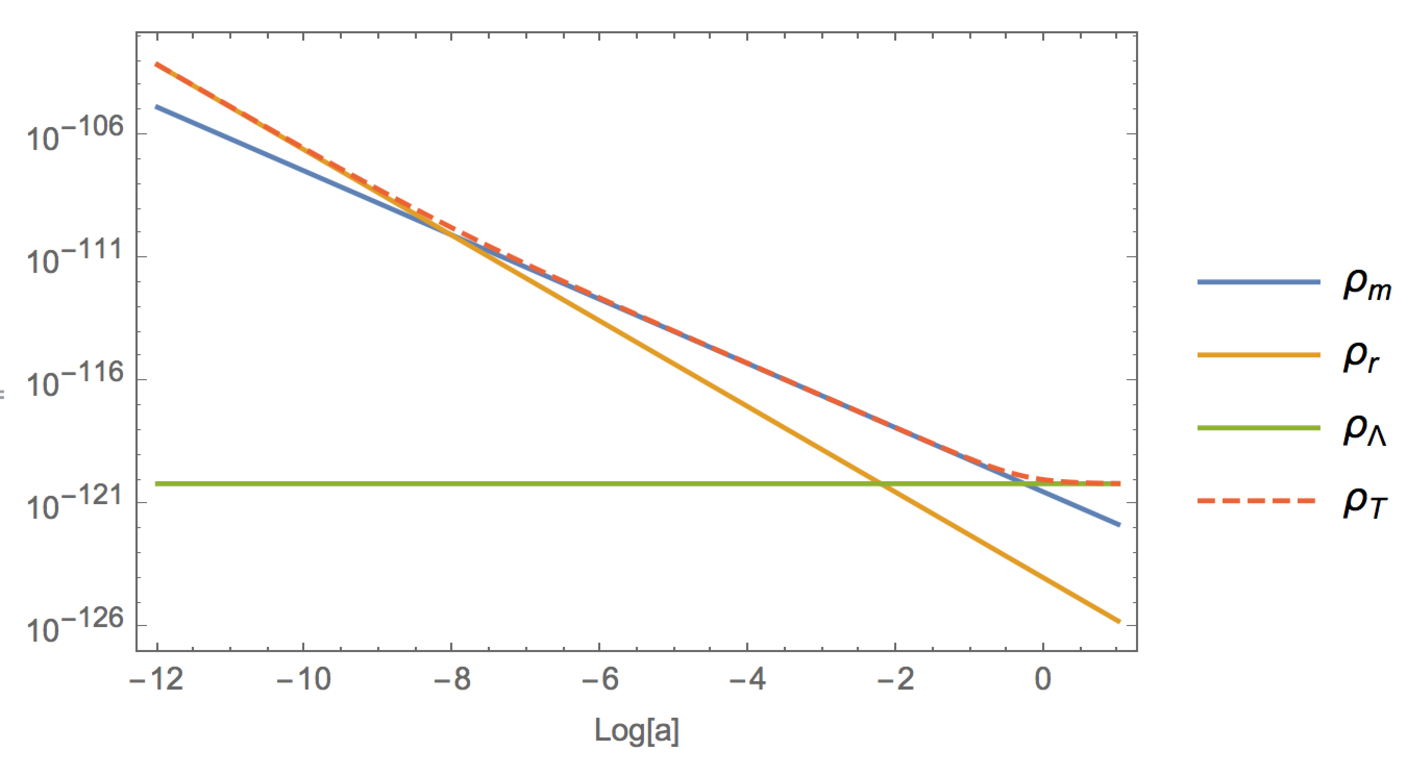
\includegraphics[width = 0.7\textwidth]{Sections/Figures/EnergyDensityEvol.pdf}
    \caption{Energy density evolution for radiation $\rho_r$, non-relativistic matter $\rho_m$, (constant) dark energy $\rho_\Lambda$ and the total energy density, $\rho_T$ as a function of the scale factor in Planck units with $a_0=1$ today.}
    \label{fig:RhoEvol}
\end{figure}


\subsection{Major Events}
\label{subsecME}

The Hot Big Bang model for cosmology assumes that the universe was initially a hot soup of elementary particles at a very high temperature. In broad terms, the subsequent  evolution describes the cooling of this hot soup as the universe expands.  Indeed, conservation of entropy (for relativistic particles with a constant number of species) implies that temperature falls as 
\be
T(t)=T_0 \left(\frac{a_0}{a(t)}\right) \,,
\ee
and can be used as an alternative to time to parameterise the history of the universe.
There are two main consequences of such an expansion and cooling:
\begin{enumerate}
\item Reaction rates in dilute systems are generically proportional to the number of participants per unit volume, because the reactants must be able to find one another before they are able to react. Since  particle densities fall as the universal volume grows, reaction rates also fall. Thus interactions between particles freeze out when the interaction rate drops below the expansion rate. This implies that one of the main trends of cosmology is that, as the universe ages, thermal and chemical reactions fall out of equilibrium.

\item A consequence of the previous point is the appearance of bound states of particles as the universe ages. Although the reactions forming bound states can always occur, at the earliest epochs temperatures are high enough to ensure that collisions very efficiently destroy these bound states, leaving very few to survive in equilibrium conditions. As the temperature drops, the inter-particle collisions become less violent and eventually the reactions of formation can dominate to leave a population of primordial relic bound states. Moreover, in an expanding universe, broken symmetries in the laws of physics may be restored at high energies. At very early epochs, phase transitions are also expected to play an important role in the cosmic evolution, but as yet there is no direct evidence that such transitions took place.
\end{enumerate}

\begin{figure}[ht]
    \centering
    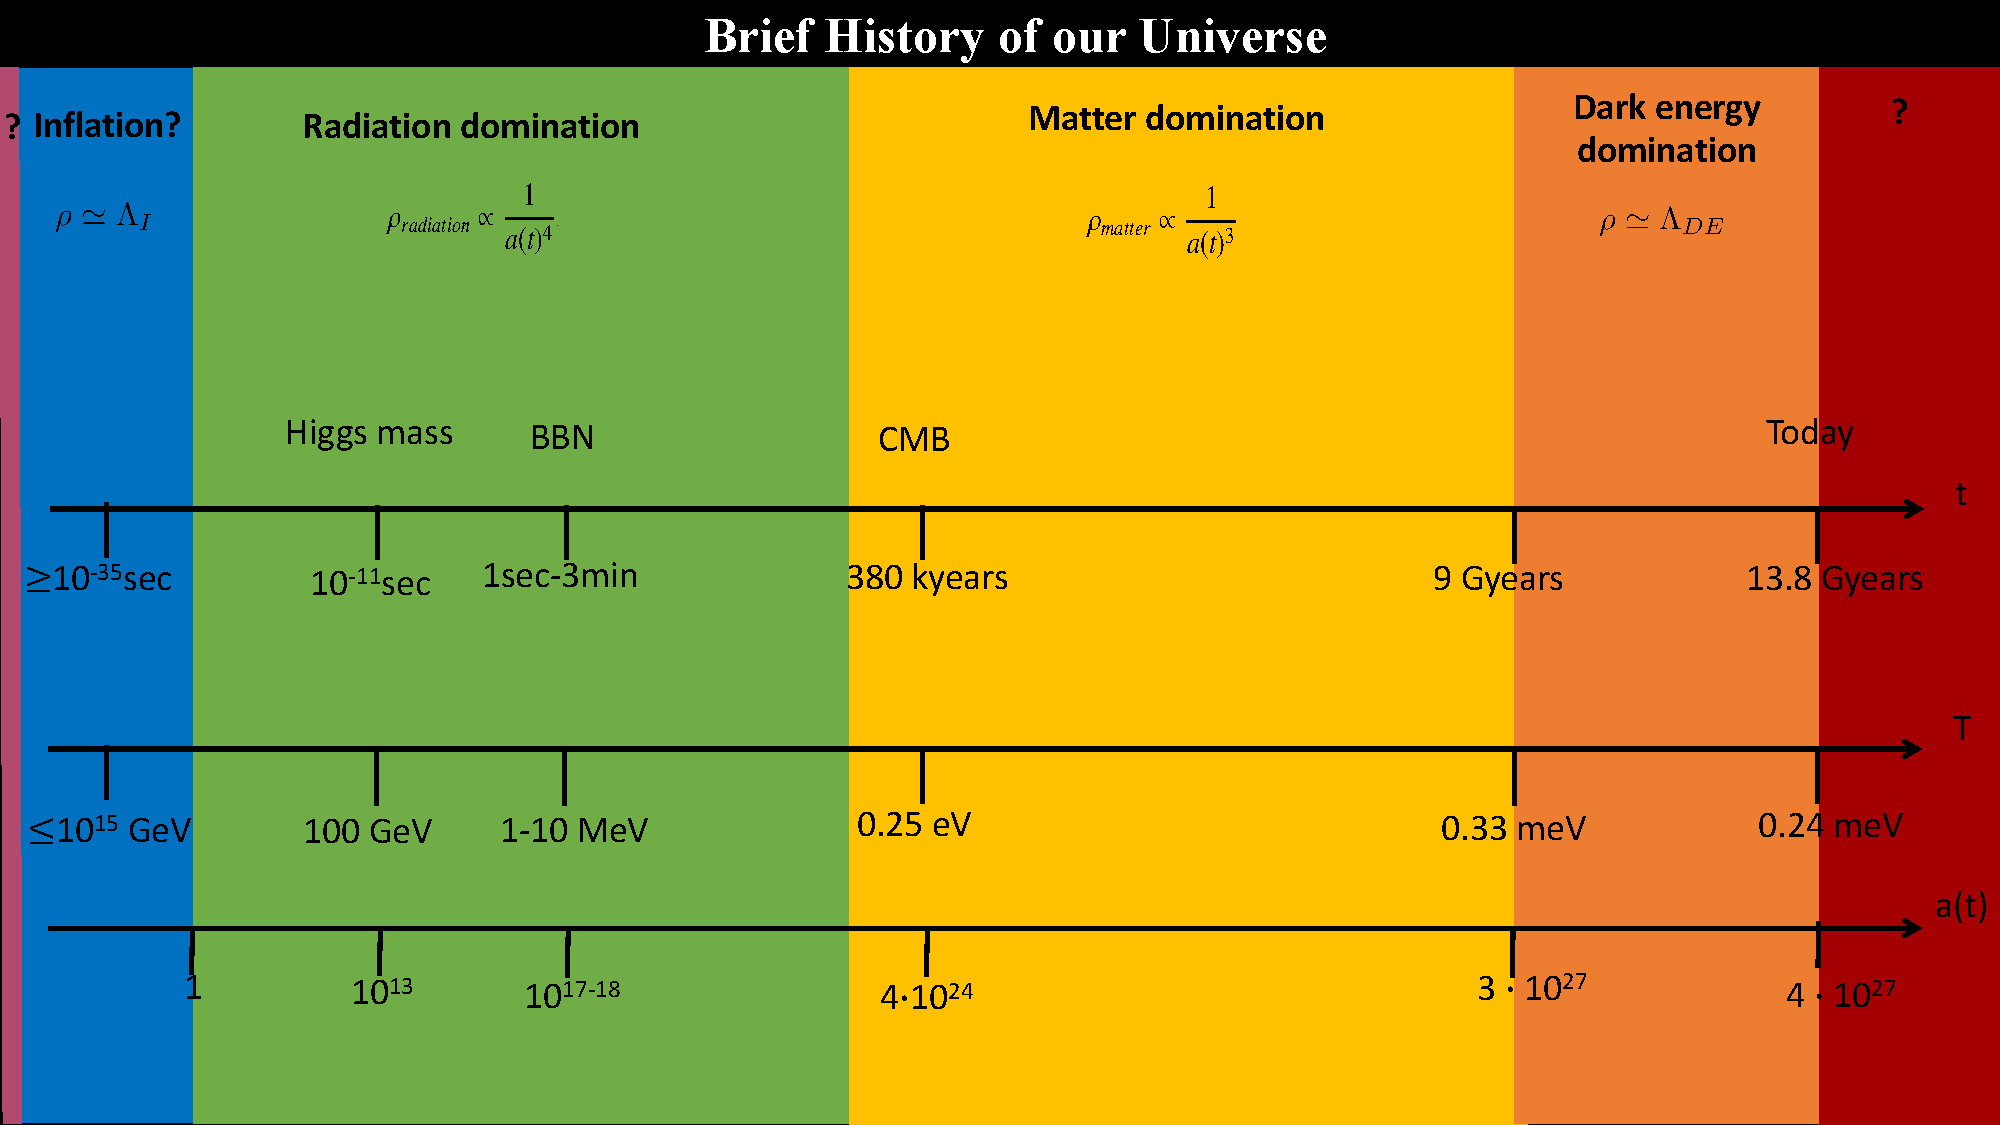
\includegraphics[width = 0.9\textwidth]{Sections/Figures/FigureHistory.pdf}
    \caption{A schematic representation of the different epochs and their temperatures within the history of the universe in
    the standard $\Lambda$CDM cosmological model.}
    \label{fig:History}
\end{figure}

The  main events constituting the history of our universe can be summarised as follows  (see Tab. \ref{tab:universe_evol} and Fig.~\ref{fig:History}).
\begin{itemize}
\item At  $t\sim 10^{-43}$ s ($10^{19}$ GeV), we are near the Planck scale, where we expect  quantum gravity effects, such as those of string theory,
to dominate and general relativity not to be valid.  One of the fundamental issues of spacetime structure at the Planckian scale is  the question of cosmic singularities.  It is expected that these problems will be  addressed in the, as yet not definitively known, non-perturbative quantum gravity theory.

\item The period from  $t\sim 10^{-43}-10^{-14}$ s corresponds to temperatures  of around $T \sim10^{19}$ GeV - $10^4$ GeV, which are not foreseeably accessible by accelerators. In this sense, the universe can be used to test fundamental physics relevant at this scales, such as supersymmetry,  grand unification, string theory, extra dimensions, and other theories. Perhaps the most interesting phenomenon in the above energy range is the accelerated expansion of the early universe, inflation, which, as will be discussed below, likely occurred  somewhere near grand unification scales.

\item The epoch from  $t\sim 10^{-14}-10^{-10}$ s, corresponding to temperatures of $T\sim 10^4$ GeV - $100$ GeV, may be accessible by accelerators.
In particular, the standard model of the electroweak and strong interactions  is applicable here.

\item At  $t\sim 10^{-5}$ s, the corresponding temperature $T\sim200$ MeV, the QCD scale, where the  quark-gluon transition takes place.

\item Between  $t\sim0.2$ s and $200-300$ s (where $T\sim 1-2$ MeV at the start and $T\sim0.05$ MeV at the end), we have temperatures at the nuclear physics scale. Two important events happen during this period. First, the primordial neutrinos decouple from the other particles and subsequently propagate without further scatterings. Second, the process of {\em primordial nucleosynthesis}  takes place.  The initial conditions for this are set by the `freeze out' of the ratio of neutrons to protons, when the interactions that keep these particles in chemical equilibrium become inefficient; the number of the surviving neutrons subsequently determines the abundances of the primordial elements. As nuclear reactions become efficient, previously free protons and neutrons form helium and other light elements. The abundances of the light elements resulting from Big Bang Nucleosynthesis (BBN) are in very good agreement with observations, and this strongly supports our understanding of the universe's evolution back to the first second after the big bang.
 
\item $t\sim10^{11}$ s ($T\sim$ eV). This time corresponds to matter-radiation equality, which separates the radiation-dominated epoch from the matter-dominated epoch.

\item  At $t\sim 10^{12}-10^{13}$ s another two related important event happens. During so-called `recombination', nearly all free electrons and protons combine to form neutral hydrogen.  At this stage, the photons decouple and the universe becomes transparent to the background radiation. The Cosmic Microwave Background (CMB) temperature fluctuations, induced by the slightly inhomogeneous matter distribution at photon decoupling, form and survive to the present day, delivering direct information about the state of the universe at the last scattering surface.

\item Finally, at our present time $t\sim 10^{16}-10^{17}$ s,  galaxies and their clusters have formed from  small primordial inhomogeneities as a result of gravitational instability. An important question regarding this period is the nature of both dark matter and also the dark energy which is driving the present day accelerated expansion.
\end{itemize}

\begin{table}
[H]
\begin{center}
\centering
\begin{tabular}{| l |  m{8em}  | m{10em}| m{10em} | m{10em} | }
\hline
\cellcolor[gray]{0.9}  {\bf Temperature} &  \cellcolor[gray]{0.9} {\bf Time }&  \cellcolor[gray]{0.9} {\bf Particle Physics } &  \cellcolor[gray]{0.9} {\bf Cosmological Event}   \\
\hline \hline
$10^{19} {\rm GeV}$   & $10^{-43} {\rm s}$ & Quantum Gravity & Gravitons decouple?   \\
\hline
$10^{19} {\rm GeV}$ -  $10^2 {\rm GeV}$   &  $10^{-43} {\rm s}$ - $10^{-12} {\rm s}$ & Grand Unification?  Desert? String theory? Extra dimensions?  &  Inflation? Topological defects? Baryogenesis?\\
\hline
 $10^2$ GeV & $10^{-12}$ s   & Electroweak Breaking & Baryogenesis?    \\
\hline
 $0.3$ GeV & $10^{-5}$ s   & QCD scale & Quark-Hadron transition    \\
\hline
 $10-0.1$ MeV & $10^{-2}$ - $10^2$ s   & Nuclear Physics Scale & Nucleosynthesis, Neutrinos decouple     \\
\hline
$10$ eV & $10^{11}$ s   & Atomic Physics Scale & Atoms formed, CMB, Matter domination     \\
\hline
\end{tabular}
\end{center}
\caption {Brief history of our universe. Temperature units can be transformed to Kelvin using the conversion factor $1\,{\rm GeV}\, =1.16 \times 10^{13}$ K.}
\label{tab:universe_evol}
\end{table}

The standard cosmological model just discussed describes a simple and consistent picture of the relatively recent universe,  which is able to account for the many available observations of the overall structure and evolution of the universe. This picture bears up to scrutiny very well, at least for all times after the epoch of BBN. This success however, comes with some drawbacks, which  can be summarised as follows:

\begin{itemize}

\item  {\em The horizon problem}.  The CMB radiation, first discovered in 1964, is known with excellent precision and  is landmark evidence of the Big Bang origin of the universe. 
One of its most striking features is that its variations in intensity across the sky are tiny, less than 0.01\% on average.
It follows from this that the universe was extremely homogeneous at the time of recombination. Assuming the standard expansion of the universe,
we receive the same physical information from causally disconnected regions of space. It is (apparently) a puzzle why the radiation is so uniform.

\item {\em The flatness problem.}  The most recent results from the CMB are consistent with a flat universe. Namely, the  position and height of the first acoustic peak on the spectrum of the CMB provides evidence for $\Omega=1$ (see \eqref{eq:OmegaGeo}) \cite{Planck:2018vyg}.
 The flatness problem refers to the fact that for $\Omega$ to be so close to one at present, it had to be essentially one in the early universe to extraordinarily high precision, which also constitutes an apparent puzzle.

\item {\em Dark matter \& Dark Energy}. The standard cosmological model, supported by the most recent data \cite{Planck:2018vyg},  postulates the existence of two new forms of matter, namely dark matter and dark energy,  for which there is  no direct evidence from particle physics or from Earth-based experiments.

\begin{itemize}

\item Dark matter: Besides CMB evidence for dark matter, the survey and study of the behaviour of matter, such as rotation curves of galaxies, at many different scales, has given evidence that there should be a new kind of matter, not present in the standard model of particle physics. This plays  an important role in the explanation of the large scale structure formation. We still do not know what dark matter is: is it a particle, or some sort of  massive compact object present in the universe?

\item Dark energy: Recent results form the study of high redshifted supernovae, combined with CMB results provide strong evidence for the fact that the universe is  accelerating today ($\ln a\sim -0.34$, see Fig. \ref{fig:RhoEvol}). This indicates that there should be a form of `dark energy' satisfying eq.~\eqref{eq:rho3p} $(\rho+3 p)<0$ and thus causing the universe to accelerate today. Either an effective cosmological constant or a time varying scalar field,
called {\em quintessence},  are the main proposals for this dark energy.
\end{itemize}
\end{itemize}

All of these problems are strong guides as to the nature of necessary extensions beyond the Hot Big Bang, and in general to the need for physics beyond that contained in the Standard Model of particle physics.

\subsection{Cosmological Inflation}
\label{sec:infla}

Cosmic Inflation was initially motivated as a way to address the flatness and horizon problems above.  Quite compellingly, it was later found that it also provides a simple explanation for the origin of the primordial density fluctuations which seeded the observed temperature fluctuations of the CMB and the formation of galaxies through gravitational collapse.

The main idea behind inflation is that the  universe underwent a period of accelerated expansion at some point in its very distant past. If the inflationary period is long enough, it rapidly flattens the universe, solving the flatness problem. It also explains why some regions could be in causal contact with each other, solving the horizon problem. Requiring that inflation solves both the flatness and horizon problems, one can estimate that inflation should last for $N\gtrsim 60$ e-foldings.

\bigskip

An accelerated expansion implies that
\be
\ddot a >0\,.
\ee
Using \eqref{eq:Hdef} we can express this condition as
\be
\label{eq:ddota}
\frac{\ddot a}{a} = H^2\lb1-\epsilon \rb >0 \,,
\ee
where we introduce the {\em slow-roll} parameter $\epsilon$, defined as
\be
\label{eq:epsdef}
\setlength\fboxsep{0.25cm}
\setlength\fboxrule{0.4pt}
\boxed{
\epsilon\equiv -\frac{\dot H}{H^2}\,,
}
\ee
and thus the condition for an accelerated universe is encoded in the requirement that
\be
\label{eq:epscond}
\epsilon<1 \,.
\ee
Using  \eqref{eq:Fried4DH} and \eqref{eq:EMconsFLRW} in \eqref{eq:epsdef}, we can write $\epsilon$ as
\be
\setlength\fboxsep{0.25cm}
\setlength\fboxrule{0.4pt}
\boxed{
\epsilon \equiv \frac{3}{2}(1+\omega)\,,
}
\ee
and thus $\epsilon <1$ implies the condition  \eqref{eq:omega_acc} for an accelerated expansion, as seen previously.

This  is equivalent to the statement that  the {\em comoving Hubble radius} $(aH)^{-1}$ shrinks in accelerated expansion,
rather than the growing behaviour of radiation and matter dominated phases. That is,
\be
\frac{d}{d t}(aH)^{-1} = -\frac{1}{a} \lb 1-\epsilon \rb <0.
\ee
In a universe dominated by a fluid with equation of state $p=\omega \rho$, the comoving Hubble radius behaves as
\be
\frac{1}{aH} \sim t^{\frac{\epsilon-1}{\epsilon}}\,,
\ee
and thus again we see that $\epsilon<1$ implies that the comoving Hubble radius decreases, while for $\epsilon>1$, it increases.
For example, during matter domination $\omega=0$ and $\epsilon = 3/2$, while during radiation domination $\omega=1/3$ and $\epsilon=2$.
Note that as soon as the condition $\epsilon<1$ fails, inflation ends and thus we can define the end of inflation as $\epsilon\sim 1$.

\begin{figure}[ht]
    \centering
    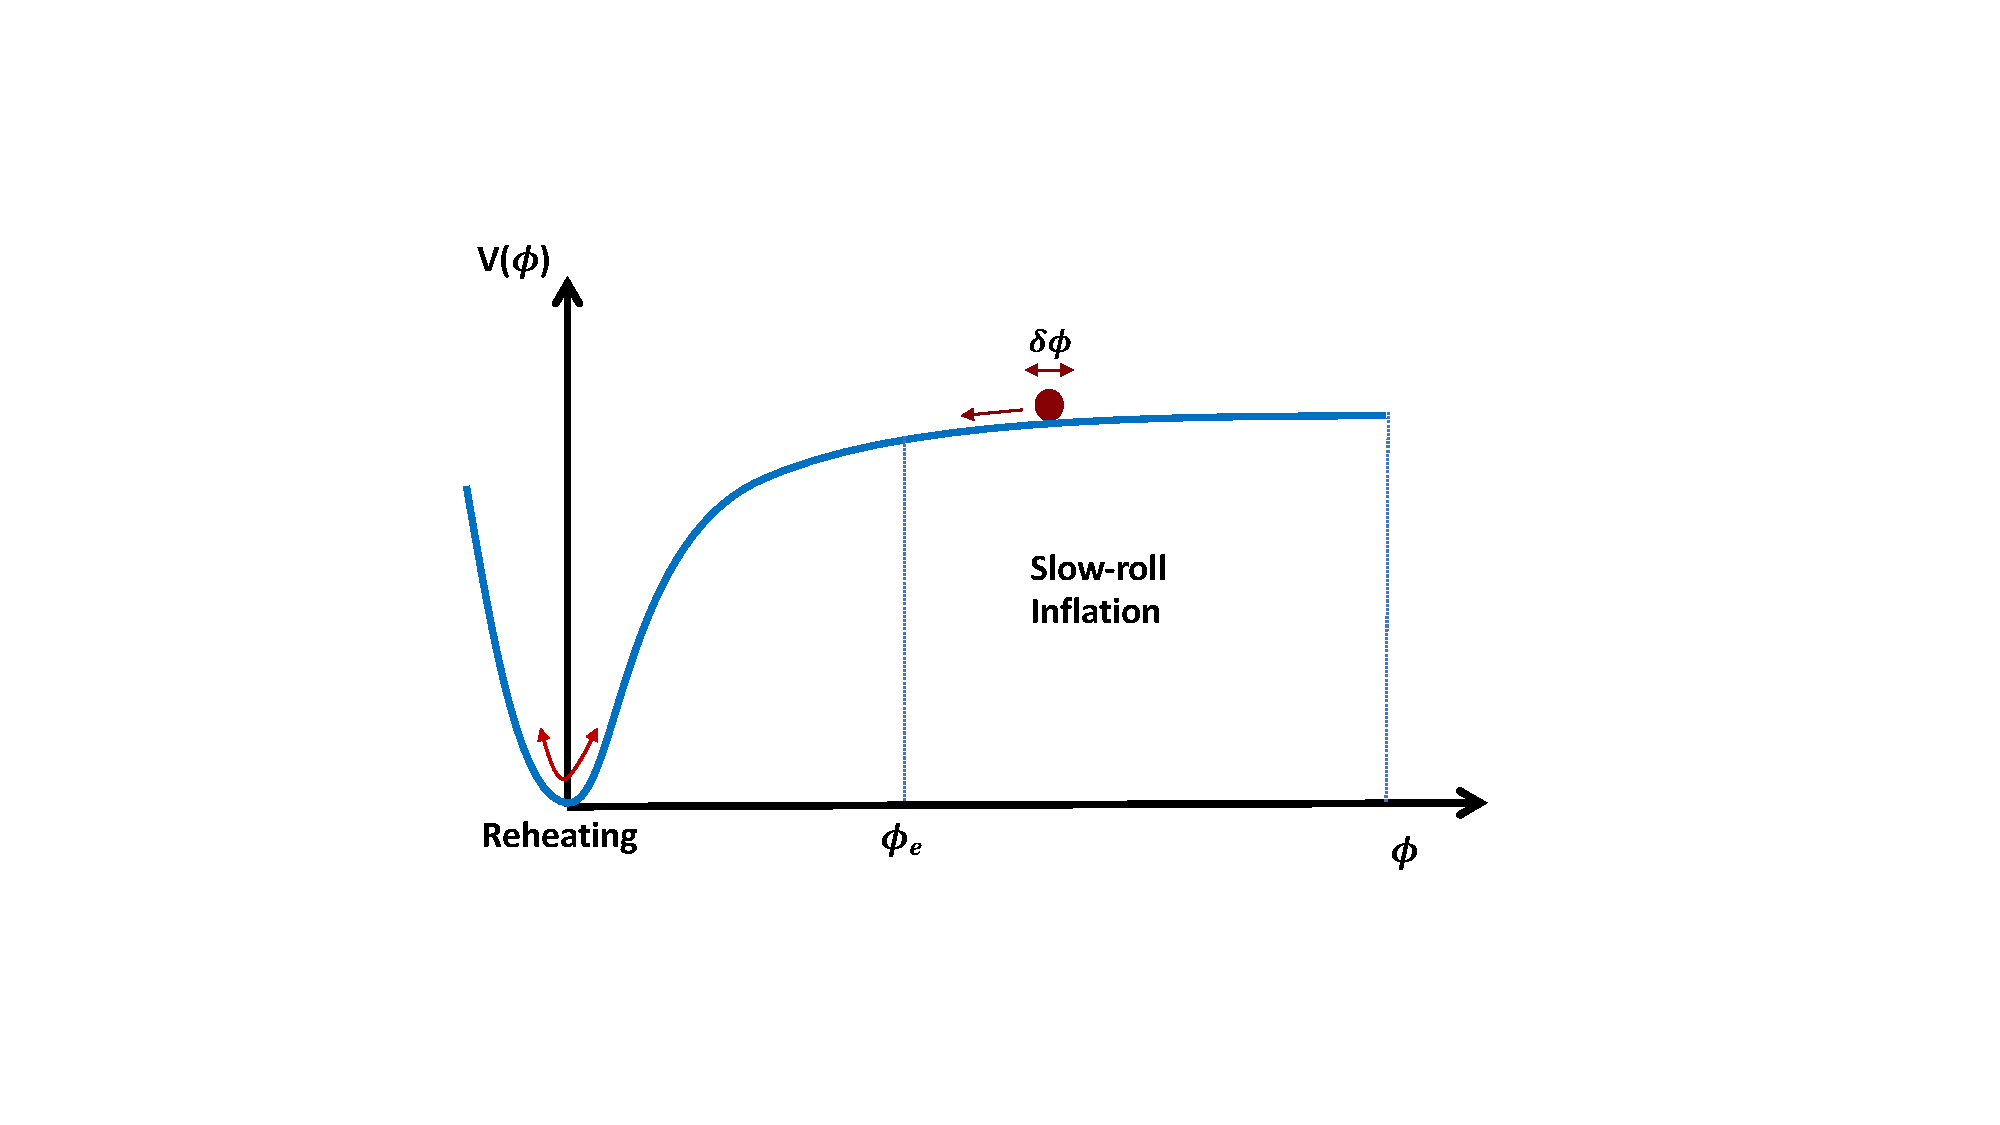
\includegraphics[width = 0.7\textwidth]{Sections/Figures/FigureInflation.pdf}
    \caption{An illustration of the standard picture of slow-roll inflation ending in fast roll of the inflation to a minimum and subsequent reheating of the universe.}
    \label{fig:Inflation}
\end{figure}

In the de Sitter limit, $\epsilon\to0$, the space grows exponentially as in \eqref{eq:dSa}. More generally, an inflationary expansion requires a somewhat unconventional matter content. Indeed, from \eqref{eq:Fried4Da} we see that, for a universe supported by a perfect fluid, the energy density and pressure should satisfy
\be
\rho+3p <0 \,,
\ee
that is, the overall pressure of the universe should be negative $p <-\rho/3$, which corresponds 
to a violation of the {\em strong energy condition} (SEC)\footnote{The SEC for a perfect fluid states that $\rho+p\geq 0$ \cite{Hawking:1973uf}.}.This occurs in neither radiation nor matter dominated phases (for which $p=\rho/3, p=0$ respectively).
However, one simple energy source that can drive inflation is the  positive potential energy  of a single (canonically normalised) scalar field with negligible kinetic energy (see Fig.~{fig:Inflation} for an illustrative example). As we will encounter later, other alternatives are also possible.

\subsubsection{Slow-roll conditions}

Let us consider a single (canonically normalised) scalar field,  {\em the  inflaton}, with potential energy $V$, coupled to gravity.  Its 
action reads
\be
\label{eq:scalarS}
S= \int{d^4x \sqrt{- g} \left[\frac{1}{8\pi\,G_4} \,\frac{R_4}{2}  - \frac{1}{2} \partial_\mu\varphi\, \partial^\mu\varphi - V(\varphi)\right]} \,.
\ee
Although the inflaton can in principle depend on both time and space, inflation rapidly smooths out spatial variations, and thus for the background evolution, it suffices to study\footnote{The spatial dependence will be relevant later for the quantum fluctuations of the inflaton.} $\varphi=\varphi(t)$.
In a spatially flat FLRW spacetime \eqref{eq:FLRW} the variation of the action \eqref{eq:scalarS} with respect to $\varphi$ gives
\be
\label{eq:phieq}
 \ddot \varphi + 3H\dot\varphi+  V_{,\varphi} =0  \,.
\ee
The energy momentum tensor of the field derived from \eqref{eq:scalarS} gives
\be
T_{\mu\nu} = \partial_\mu\varphi\partial_\nu\varphi -g_{\mu\nu}\lb \frac12 (\partial\varphi)^2 +V(\varphi)\rb\,.
\ee
In the flat FLRW background, the energy density and pressure of the scalar are found to be
\begin{subequations}
 \begin{align}
 \label{eq:rhoscalar}
\rho_\varphi& = \frac{1}{2} \dot \varphi^2 +V(\varphi)\,, \\
p_\varphi &= \frac{1}{2} \dot \varphi^2 -V(\varphi)\,.\label{eq:Pscalar}
\end{align}
\end{subequations}
With this, eqs. \eqref{eq:Fried4DH} and \eqref{eq:Fried4Da} yield
\bea
&&H^2 = \frac{8\pi\,G_4}{3} \left(\frac{\dot \varphi^2}{2}  + V(\varphi)\right) \,, \label{eq:Hscalar} \\
&& \frac{\ddot a}{a} = -\frac{8\pi\,G_4}{3} \lp \dot\varphi^2 -V(\varphi) \rp  \,.
\label{eq:Rayscalar}
\eea
We now introduce the slow-roll conditions. A nearly exponential expansion can be ensured by the requirement that the fractional change of the Hubble
parameter per e-fold $N$ is small, that is $\epsilon \ll1 $ (see eq.~\eqref{eq:epsdef}). In terms of the inflaton,
$\varphi$, this can be written as (from now on we use $\Mp$ rather than $G_4$)
\be
\label{eq:epsfi}
\epsilon = \frac{\dot\varphi^2}{2 \Mp^2 H^2} \ll 1\,.
\ee
Requiring that inflation lasts for a sufficiently long time that the horizon problem is solved is equivalent to requiring that $\epsilon$ remain small for a sufficient number of Hubble times, which is measured by the {\em second slow-roll} parameter, $\eta$, defined as
\be
\label{eq:etafi}
\setlength\fboxsep{0.25cm}
\setlength\fboxrule{0.4pt}
\boxed{
\eta\equiv \frac{\dot \epsilon}{H\epsilon} = \frac{\ddot H}{H\dot H} + 2\epsilon = 2\frac{\ddot \varphi}{H\varphi} + 2\epsilon\,.
}
\ee
This then implies that $\delta_\varphi\ll1$, where we defined 
\be
\label{eq:deltafi}
\setlength\fboxsep{0.25cm}
\setlength\fboxrule{0.4pt}
\boxed{
\delta_\varphi \equiv \frac{\ddot \varphi}{H\dot\varphi}  \,.
}
\ee
 Using the Friedman equation \eqref{eq:Hscalar}, we  see that the first slow-roll condition \eqref{eq:epsfi}, implies
that $\dot\varphi^2 \ll V$ and therefore we can write \eqref{eq:Hscalar} as
\be
\label{eq:Hslowr}
H^2 \simeq \frac{V(\varphi)}{3 \Mp^2} \,.
\ee
Moreover, using \eqref{eq:deltafi}, we can write \eqref{eq:phieq} as
\be
\label{eq:fislowr}
3H\dot \varphi + V_{,\varphi} \simeq0\,.
 \ee

In the present case of a single scalar field, we can write the slow-roll conditions \eqref{eq:epsfi} and \eqref{eq:deltafi} (equivalently \eqref{eq:etafi}) solely in terms of the scalar potential and its derivatives as follows.  From the condition \eqref{eq:epsfi}, using \eqref{eq:fislowr} and \eqref{eq:Hslowr}, we arrive at
\be\label{eq:epsV}
\setlength\fboxsep{0.25cm}
\setlength\fboxrule{0.4pt}
\boxed{
  \epsilon_V\equiv \frac{\Mp^2}{2} \lp\frac{V_{,\varphi}}{V}\rp^2 \simeq \epsilon \,,
  }
\ee
which is the first {\em potential slow-roll parameter}.
Next, using the conditions \eqref{eq:fislowr} and  \eqref{eq:Hslowr} in \eqref{eq:deltafi}, we obtain
\be
\Mp^2 \frac{V_{,\varphi\varphi}}{V} + \epsilon \ll 1\,,
\ee
and so therefore introduce the second potential slow-roll parameter,  $\eta_V$,
\be\label{eq:etaV}
\setlength\fboxsep{0.25cm}
\setlength\fboxrule{0.4pt}
\boxed{
\eta_V \equiv \Mp^2 \,\Bigg|\frac{V_{,\varphi\varphi}}{V} \Bigg|\,.
}
\ee
Thus, {\em in single field inflation}, the slow-roll parameters can be written in terms of the scalar potential and its derivatives, which need to be  small during  inflation:
\be
\epsilon_V \ll1 \,,\qquad \eta_V\ll1 \,.
\ee
Note that in this case, the smallness of the $\eta_V$-parameter (which in the present single field case is equivalent to $\eta$ and $\delta_\varphi$),  implies that the mass of the inflation, $|m_{\rm inf}^2| \sim |V_{,\varphi\varphi}| \ll H^2$ 
(as we will see, this conclusion no longer holds when more scalar fields are present \cite{Chakraborty:2019dfh,Aragam:2021scu}). The required smallness of the slow-roll parameters, and in particular the mass of the inflaton, is vulnerable to quantum corrections, as we will discuss in detail when we consider UV complete models in Sec. \ref{sec:infla}.

\subsubsection{Primordial fluctuations}\label{sec:PrimF}

As we have seen, the early universe is supposed to have been rendered very nearly uniform by a primordial inflationary epoch. According to our current understanding, structures in the universe originated from tiny `seed' perturbations, which grew to form  all the structures we observe today.
Observations of the CMB support this view, indicating that at the time of decoupling the universe was very nearly homogeneous with small inhomogeneities at the $10^{-5}$ level.
The best candidate for the origin of these perturbations is quantum fluctuations produced during  inflation  in the early universe.
 These perturbations extend from extremely short scales to cosmological scales by the stretching of space during inflation.
%
\begin{center}
\begin{figure}[H]
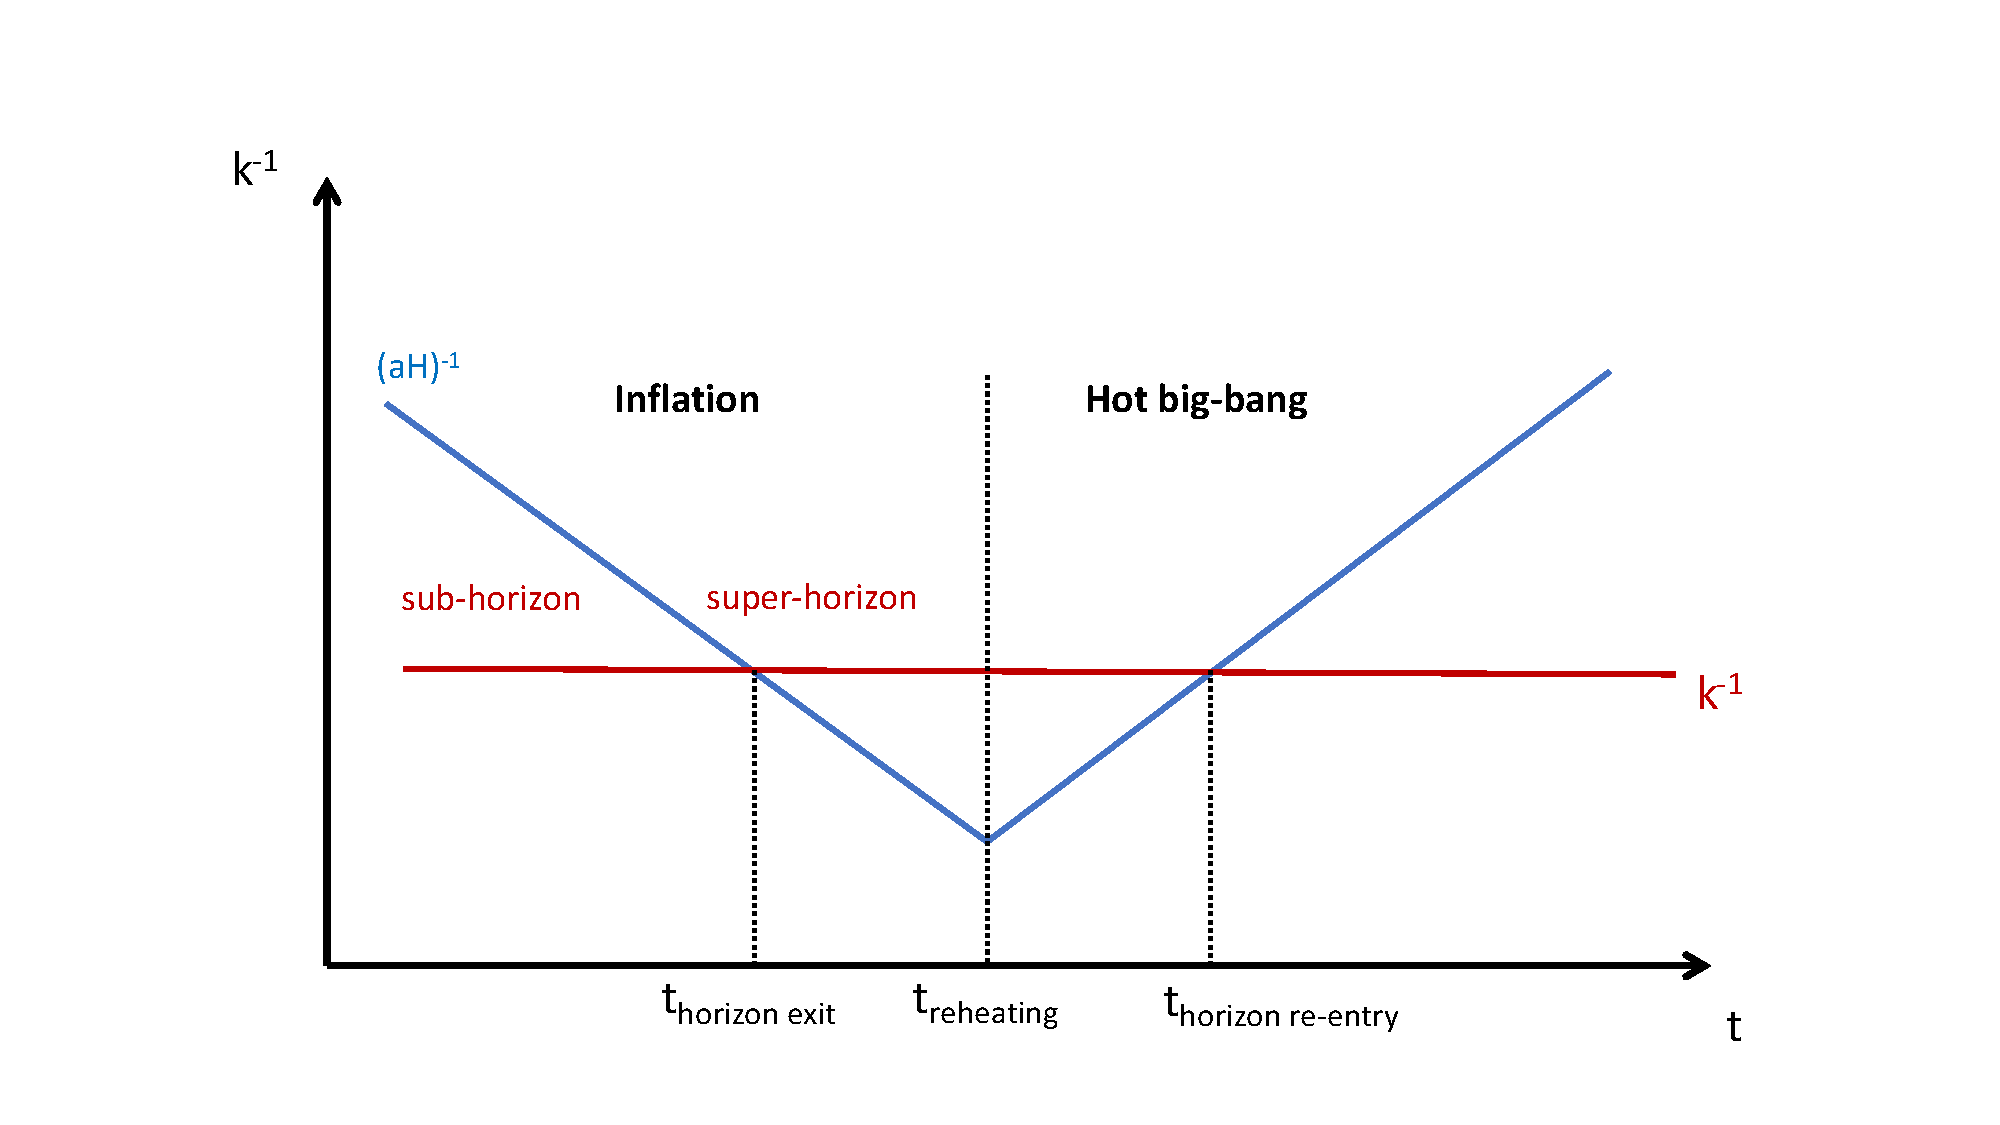
\includegraphics[width=14cm]{Sections/Figures/DensityPerturbations.pdf}
\caption{Horizon exit and re-entry of a density perturbation with wave number $k$.}
\label{Fig:perturbations}
\end{figure}
\end{center}
%
The shrinking of the comoving Hubble radius (Hubble horizon) during inflation implies that fluctuations leave the horizon at some point (see Fig.~\ref{Fig:perturbations}).  Once inflation  ends,  the Hubble radius increases and  the fluctuations eventually reenter it during the radiation -- or matter -- dominated epochs. Fluctuations that exit the horizon around 60 e-foldings or so before the end of inflation, reenter with physical wavelengths in the range accessible to cosmological observations, with the CMB probing around 7-10 e-folds (note that the number 60 here depends on the post-inflationary evolution which, as discussed in Sec. \ref{reheating}, can be quite different in stringy scenarios compared to the vanilla picture of immediate reheating; see \cite{Bhattacharya:2017ysa, Bhattacharya:2017pws} for discussions in a stringy context). The spectra generated for density perturbations and gravitational waves during inflation provide a distinctive signature and can be measured by analysing the microwave background radiation anisotropies.


During inflation,  the inflaton field dominates the energy density of the universe, and thus any perturbation on it  implies  a perturbation of the  energy-momentum tensor
\be
\delta\varphi \quad  \Longleftrightarrow  \quad \delta T^{\mu\nu}\,.
\ee
A perturbation in the energy-momentum tensor then implies, via Einstein's equations of motion, a perturbation of the metric
\be
\delta G_{\mu\nu} =  \lp \delta(R_{\mu\nu}) -\frac12\delta(g_{\mu\nu}\,R)\rp = 8\pi G \delta T^{\mu\nu} \, ,
\ee
and so we have
\be
\delta\varphi \quad  \Longleftrightarrow \quad \delta g_{\mu\nu}\,.
\ee
The metric perturbations can be decomposed according to their spin into {\em scalar}, {\em vector} and {\em tensor} perturbations with respect to rotations of spatial coordinates on hypersurfaces of constant time. At  linear order, the scalar, vector and tensor perturbations evolve independently (decouple) and it is thus possible to analyse them separately. Vector perturbations do not get excited during inflation because there are no rotational velocity fields. In what follows, we summarise the analysis of scalar and tensor perturbations in inflation. For more details see e.g.~\cite{Mukhanov:1990me,Riotto:2002yw}.

\subsubsection*{Gauge choice}

An important  subtlety in the study of cosmological perturbations is that  the split into background and perturbations  is not unique, but depends on the choice of coordinates or the gauge choice.  It is important to note that there is no preferred gauge.  
To eliminate this ambiguity, one has two choices:
either identify  {\em gauge invariant} quantities or choose a given gauge and perform the calculations in that gauge.
Both options have advantages and drawbacks. By selecting a certain gauge, the calculations might be made technically simpler, but there is a risk that doing so introduces gauge artifacts or unphysical perturbations. On the other hand, a gauge-invariant computation may be technically more involved, but has the advantage of dealing only with physical quantities.

\subsubsection*{Gauge-invariant variables}

As we discussed above, it is helpful to provide gauge-invariant combinations of metric and matter perturbations in order to avoid the problem of spurious gauge modes. There are three gauge invariant quantities that are usually  defined in calculations of inflation: \\

\begin{tcolorbox}[title={\bf Gauge invariant variables}]

\begin{enumerate}[i.]
\item The {\em comoving curvature perturbation}. This is given by
\be\label{eq:curvatureR}
{\cal R} =\Psi + H\, \frac{\delta\varphi}{\dot\varphi} \,,
\ee
where $\Psi$ is the spatial {\em curvature perturbation}. In geometrical terms, $\cal R$  measures the spatial curvature of comoving hypersurfaces.

\item The {\em curvature perturbation on slices of uniform energy density}. This is given by
\be
\zeta = \Psi -\frac{\delta\rho}{3(\rho+p)}\,.
\ee
Geometrically, $\zeta$ measures the spatial curvature of constant-density hypersurfaces.
 For a scalar field, $(\rho+p) =\dot\varphi^2$. Moreover, during inflation   $\delta\rho \simeq-3H\,\dot\varphi\,\delta \varphi$.  Thus
 $\zeta$ and $\cal R$ are  equal during slow-roll inflation. As we will see they are also equal on {\em super-horizon scales} and therefore the correlation functions of $\zeta$ and $\cal R$ are  the same at horizon crossing. Moreover,  both  are conserved on super-horizon scales during slow-roll inflation.

\item Scalar field perturbations in  {\em spatially flat gauge}. The {\em spatially flat gauge} is defined as the slicing where there is no curvature $\Psi=0$. It gives a  gauge-invariant measure of inflaton perturbations and is given by
\be
Q = \delta\varphi +\frac{\dot\varphi}{H}\,\Psi \,. 
\ee


\end{enumerate}

\end{tcolorbox}

\bigskip
One can compute the curvature perturbation generated during inflation on super-Hubble scales,  $\zeta$ or ${\cal R}$, either using a particular gauge and computing the gauge-invariant curvature in that gauge, or by doing a fully gauge-invariant calculation. The results are equivalent.

The gauge-invariant curvature perturbation $\cal R$ defined above   is conserved outside of the horizon. Thus, we can compute it   at {\em horizon exit} and remain ignorant about the sub-horizon physics during and after {\em reheating} until horizon re-entry of a given $\cal R$-mode, $k$.

The equation of motion for the curvature perturbation $\cal R$, takes a simple harmonic oscillator form  and thus it can be quantised by promoting the classical field $\cal R$ to a quantum operator and then quantising it. One can then compute the power spectrum of curvature fluctuations at horizon crossing.

We summarise the results and refer the reader to the bibliography for the details on the computations \cite{Riotto:2002yw}. 


\subsubsection*{Scalar perturbations}

The mode equation of motion for the Fourier components of $\cal R$ is given by
\be
\label{eq:R}
\setlength\fboxsep{0.25cm}
\setlength\fboxrule{0.4pt}
\boxed{
\cR''_k + 2\frac{z'}{z}\,\cR_k'+k^2\,\cR_k=0\,,
}
\ee
where here a prime denotes derivative with respect to  conformal time
$\eta$, $d\eta = dt/a(t)$; $k$ is the wavenumber and $z\equiv a\,\dot\varphi/H$, sometimes referred to as the {\em pump field}, which satisfies
\be
\label{eq:pumpf}
\setlength\fboxsep{0.25cm}
\setlength\fboxrule{0.4pt}
\boxed{
\frac{z'}{z} = aH\lp 1+\epsilon-\delta\rp\,,
}
\ee
where we have defined\footnote{Note from \eqref{eq:etafi} that $\eta=-2\delta+2\epsilon$. Note also the difference between $\delta$, determined by the full energy density and $\delta_\varphi$, which is associated only to the dynamics of a scalar fluid(s) component.}
\be
\setlength\fboxsep{0.25cm}
\setlength\fboxrule{0.4pt}
\boxed{
\delta\equiv -\frac{\ddot H}{2H\dot H}\,.
}
\ee
Let us note that fluctuations are created on all length scales, $\lambda$.
Relating the length scale  with its wavenumber $k$, as $\lambda = 2\pi a/k$
this means that the fluctuations are created with a spectrum of wavenumbers, $k$. Fluctuations that are cosmologically relevant start their lives inside the horizon (i.e.~Hubble radius), that is $k/aH\gg 1$.
However, while the comoving wavenumber is constant the comoving Hubble radius shrinks during  inflation. Scales for 
which  $k/aH\ll 1$ are outside the Hubble radius; eventually, all fluctuations exit the horizon. Thus we refer to the scales as follows (see Fig.~\ref{Fig:perturbations}):

\begin{subequations}\label{eq:scales}
\begin{empheq}[box=\widefbox]{align}
 &\frac{k}{aH}\gg 1 \qquad \Rightarrow \qquad \text{sub-horizon scales} \nonumber\\
&\frac{k}{aH}\ll 1 \qquad \Rightarrow \qquad \text{super-horizon scales} \nonumber
\end{empheq}
\end{subequations}

\ni For scales well outside the horizon, the solutions to \eqref{eq:R} are given by
\be
\label{eq:Rsuperhor}
\cR_k(\eta) = \cC_1 + \cC_2 \int\frac{d\eta}{z^2}\,,
\ee
where $\cC_1$ and $\cC_2$ are integration constants. From \eqref{eq:pumpf} we have
\be\label{eq:zsol}
z(a) = z_0 \,{\rm exp}\lb \int{ (1+\epsilon-\delta) \,d\ln a}\rb\,,
\ee
and therefore we see that during slow-roll,  when $\epsilon, \delta\ll 1$, $z\sim a$. Since  in this case $a\sim -1/(H\eta)$ we see that the term proportional to $\cC_2$ in \eqref{eq:Rsuperhor} decays rapidly as $a^{-3}$  outside the horizon, and is thus called the {\em decaying mode}. The  curvature perturbation is conserved at super-horizon scales and controlled by the {\em constant mode} $\cC_1$.
We thus see that the constancy of ${\cal R}_k$ depends on $\epsilon$ and $\delta$ doing nothing dramatic even after horizon crossing.
However, a more dramatic situation can  arise from a failure of slow-roll. If at any time after horizon crossing the friction term in \eqref{eq:R} changes sign,  becoming a negative driving term, the decaying mode can become a growing mode with interesting cosmological implications \cite{Leach:2000yw,Leach:2001zf,Ozsoy:2018flq}. This change of sign can occur whenever $z$ reaches a local maximum, that is,  whenever $1+\epsilon-\delta=0$. Since $\epsilon$ is always positive, $\delta$ must be at least one for this to happen. This can occur during a transient period of fast-roll, ultra slow-roll  or non slow-roll period. We review below briefly this possibility.

The  amplitude of the scalar power spectrum at leading order in slow-roll can be obtained by matching the super-horizon solution with the Bunch-Davies vacuum at sub-horizon scales, to obtain\footnote{This is sometimes denoted as $\cP_\cR$ or $\Delta_s$.}:
\be
\setlength\fboxsep{0.25cm}
\setlength\fboxrule{0.4pt}
\boxed{
\cP_\cR = \frac{ H^4}{(2\pi)^2\,\dot\varphi^2}\,\Bigg|_{k=aH} = \frac{H^2}{8\pi^2\Mp^2 \,\epsilon }\,\Bigg|_{k=aH}\,,}
\ee
where all quantities are evaluated at {\em horizon crossing}, $k=aH$ and we have used \eqref{eq:epsfi} in the last equality. The power spectrum of the  cosmic microwave background scalar fluctuations is shown in Figure \ref{Fig:Spectrum}. 

\begin{figure}[t]
\begin{center}
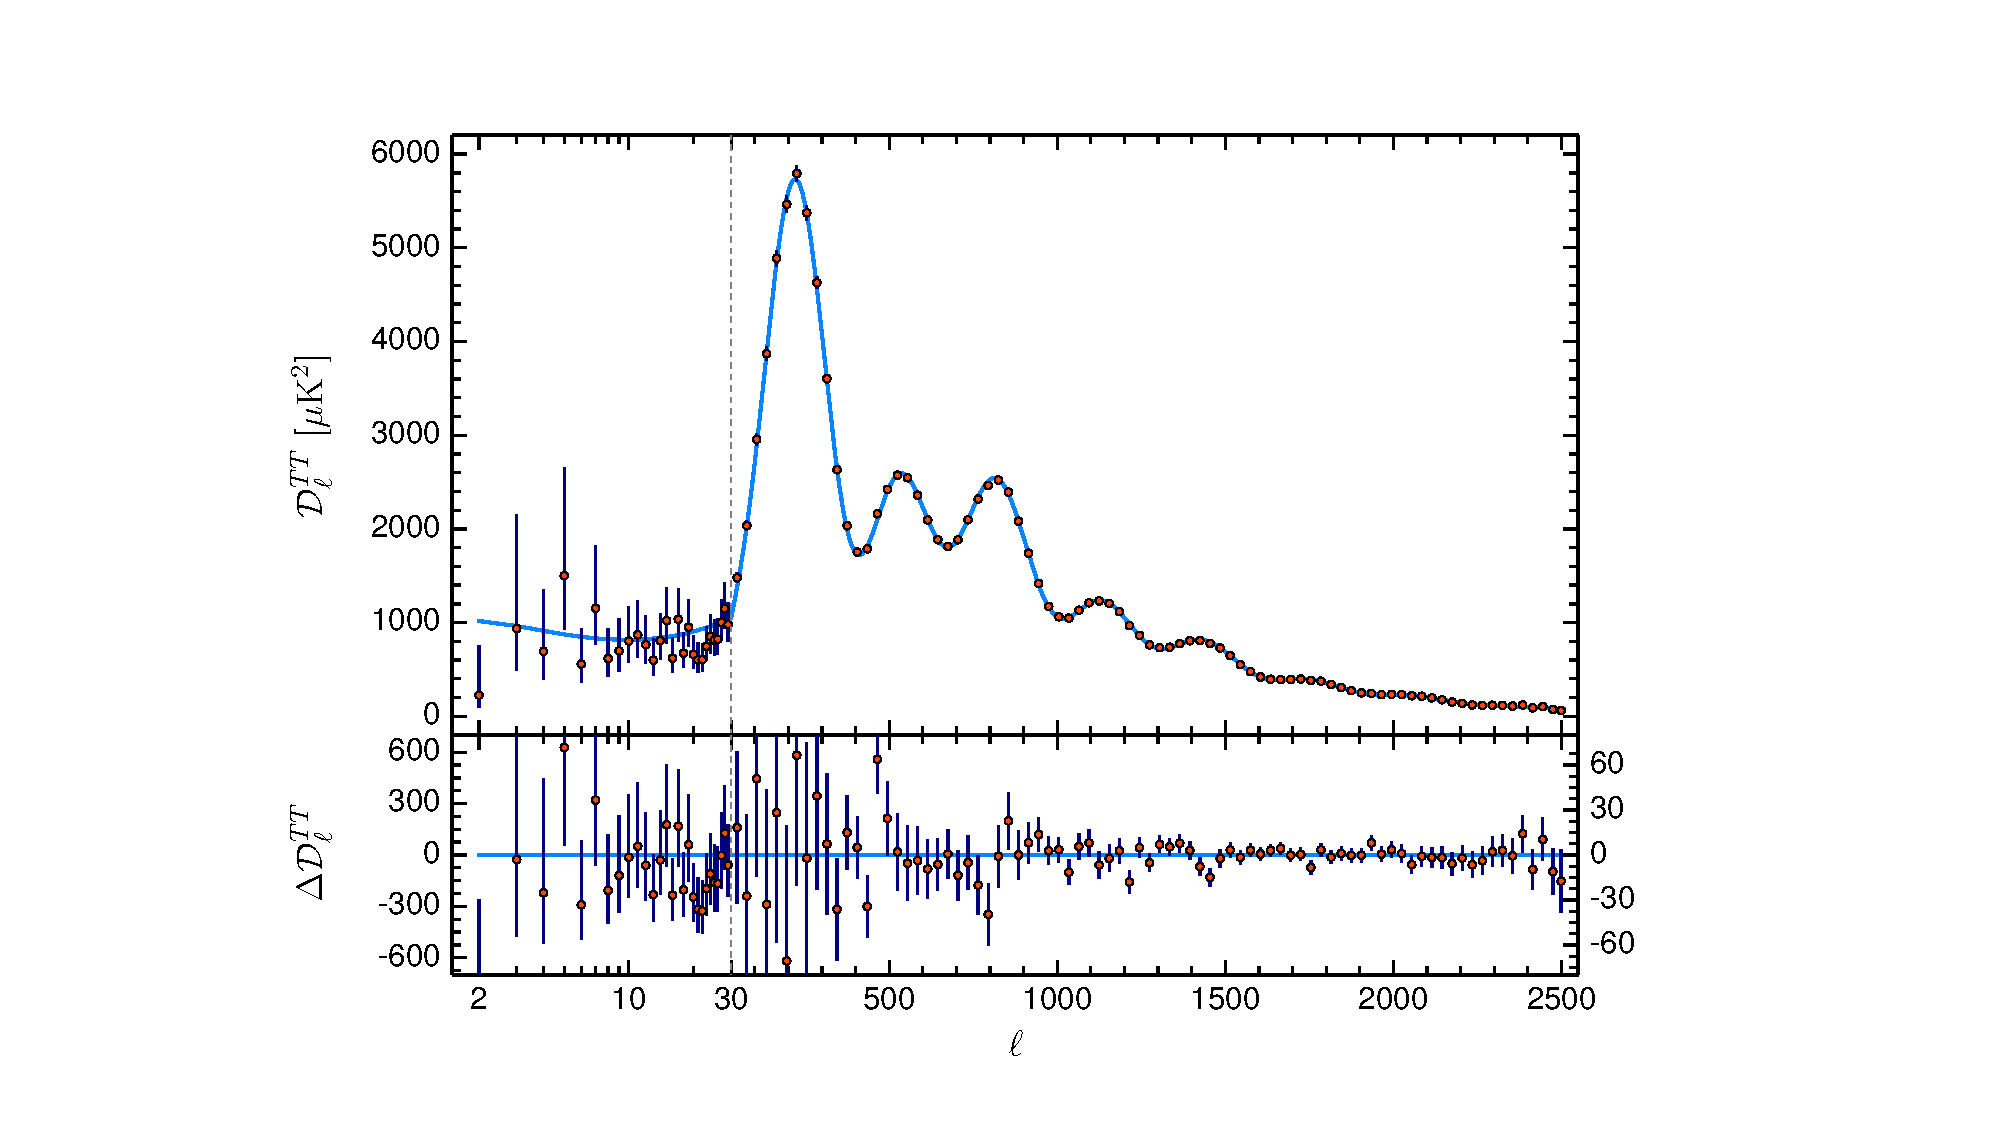
\includegraphics[width=145mm,height=105mm]{Sections/Figures/CMBSpectrum.pdf} 
\caption{The power spectrum of the scalar fluctuations of the cosmic microwave background including error bars for the $\Lambda$CDM model. This is one of most impressive examples of the precision level ($\simeq 10^{-5}$)  reached in cosmology so far, in which only a handful of parameters is enough to explain such a large number of data points (taken from \cite{Planck:2018vyg}). } \label{Fig:Spectrum} 
\end{center}
\end{figure}


\subsubsection*{Primordial tensor perturbations}

Quantum fluctuations in the gravitational field are generated in a similar fashion as the scalar perturbations discussed so far.
In general, the linear tensor perturbations may be written as
\be
ds^2 = a^2(\eta)\lb -d\eta^2 +(\delta_{ij}+h_{ij}) dx^idx^j\rb\,,
\ee
with $h_{ij}\ll1$. If the energy momentum tensor is diagonal, as is the case in the simplest inflationary model we have discussed so far,  the tensor modes do not have any source and their action is that of two (not yet canonically normalised) independent massless scalar fields\footnote{The tensor $h_{ij}$ has six degrees of freedom, but  tensor perturbations are traceless,  $h^i_i=0$, and transverse $\partial^ih_{ij}=0,  (i = 1,2,3)$. These are four constraints, that leave only  two physical degrees of freedom, or polarisations.}.

The corresponding canonically normalised field (dropping $ij$ indices),
\be
v_k \equiv  \frac{a}{2}\Mp \, h_k\,,
\ee
satisfies the equation of motion
\be
\label{eq:tensoreq}
v_k'' +\lp k^2 -\frac{a''}{a}\rp v_k =0\,,
\ee
which is the equation of motion of a massless scalar field  in a quasi-de Sitter epoch. It is interesting to note that, contrary to the scalar case, no  interesting effects arising from transient violations of slow-roll can occur for gravitational waves in standard GR.\footnote{However, in general scalar-tensor theories there can be non-trivial effects as discussed in \cite{Mylova:2018yap}.} This can be most easily seen as follows. Defining the field
\be
\psi_k = \frac{v_k}{a}\,,
\ee
Eq.~\eqref{eq:tensoreq} becomes
\be\label{eq:tensoreq2}
\psi_k'' + 2 aH \psi_k' + k^2 \psi_k =0\,.
\ee
As the `pump field' $a$ increases for all time, the constancy of the gravitational wave amplitude after horizon crossing is guaranteed until horizon re-entry \cite{Leach:2000yw}.

The  amplitude of the tensor power spectrum is  found to be
\be\label{eq:PT}
\setlength\fboxsep{0.25cm}
\setlength\fboxrule{0.4pt}
\boxed{
\cP_T = \frac{2}{\pi^2}\frac{H^2}{\Mp^2}\Bigg|_{k=aH}\,.}
\ee
Note that  this differs from the scalar power spectrum by depending only on the value of $H$ and not additionally on the slow-roll parameter $\epsilon$. Consequently, a comparison of both scalar and tensor modes  amplitudes provides a direct measure of the slow-roll parameter $\epsilon$. A more precise statement of this comparison is usually phrased in terms of the parameter $r$, defined as {\em tensor-to-scalar ratio} of the power spectra
\be\label{eq:rdef}
\setlength\fboxsep{0.25cm}
\setlength\fboxrule{0.4pt}
\boxed{
r\equiv \frac{\cP_T}{\cP_\cR} = 16 \,\epsilon\,.
}
\ee

\subsubsection{Scale dependence}

The scale dependence of the power spectra  is given by the spectral tilt indices and follows from the time-dependence of the Hubble parameter. The  scalar and tensor spectral indices are given, respectively, by
\be
\setlength\fboxsep{0.25cm}
\setlength\fboxrule{0.4pt}
\boxed{
n_s -1 \equiv \frac{d\ln \cP_\cR}{d\ln k} \,, \qquad \qquad n_t \equiv \frac{d\ln \cP_T }{d\ln k}\,.
}
\ee
Using that $d\ln k = H dt + d (\ln H)$ one finds, to first order in the Hubble slow-roll parameters
\begin{subequations}
\label{eq:nsnT}
\begin{empheq}[box=\widefbox]{align}
 n_s-1 &= -2\epsilon -\eta  \,,\\
n_T &= -2\epsilon\,,
\end{empheq}
\end{subequations}
where $\epsilon, \eta$ are defined in eqs.~\eqref{eq:epsdef} and \eqref{eq:etafi} respectively and these quantities are defined at horizon crossing.

We see that single-field slow-roll models satisfy a {\em consistency condition} between the tensor-to-scalar ratio $r$ and the tensor tilt $n_T$:
\be\label{eq:ccinfla}
\setlength\fboxsep{0.25cm}
\setlength\fboxrule{0.4pt}
\boxed{
r=-8\, n_T \,.
}
\ee
 If this relation were to be falsified by future observations of the CMB anisotropies, it would indicate that inflation was not driven by a single field.

 \subsubsection{Lyth bound}

Note that from eqs.~\eqref{eq:rdef} and \eqref{eq:epsfi}, we see that  the tensor-to-scalar ratio relates directly to the evolution of the inflaton as a function of the number of e-foldings $N=\int H dt$:
 \be
 r = \frac{8}{\Mp^2} \lp\frac{d\varphi}{dN}\rp^2\,.
 \ee
 Therefore,  the total field evolution, between the time when CMB fluctuations left the horizon at $N_{\rm hc}$ and the end of inflation at $N_{\rm end}$, is given by
 \be
 \frac{\Delta\varphi}{\Mp} = \int^{N_{\rm hc}}_{N_{\rm end}}{ dN \,\sqrt{\frac{r}{8}} } \,.
 \label{LythBound}
 \ee
 Making the conservative assumption that $r$ remains approximately constant during the inflationary period probed by the CMB, the inflaton must satisfy the so-called {\em Lyth bound} \footnote{Taking into account that the fact that $r$ does not
remain constant gives a much stronger bound \cite{Garcia-Bellido:2014wfa}.} \cite{Lyth:1996im,Boubekeur:2005zm}:
\be\label{eq:Lythbd}
\setlength\fboxsep{0.25cm}
\setlength\fboxrule{0.4pt}
\boxed{
\frac{\Delta\varphi}{\Mp} \gtrsim  \,2\times \lp\frac{r}{0.01} \rp^{1/2}\,.
}
\ee
This relation indicates that `large' values of the tensor-to-scalar ratio, $r \sim 0.01$, correlate with $\Delta\varphi \sim \Mp$, or {\em large-field inflation}. The vulnerability of large-field inflation to quantum corrections will be discussed in Sec. \ref{sec:infla}.

Using Eqs. \eqref{eq:PT} and \eqref{eq:rdef}, one can also immediately relate the Hubble parameter during inflation to the tensor-to-scalar ratio or slow-roll parameter $\epsilon$:
\be
H_{\rm inf} = \sqrt{8 \pi^2 \cP_\cR\,\epsilon}\, \Mp \,.
\ee
The observational constraints that we are about to summarise might then make a high GUT-scale, large-field inflation seem more likely in the context of a single inflaton field.

\subsubsection{Current inflationary constraints}

In this section we summarise the most recent CMB experimental results that have tested the physics of inflation \cite{Planck:2018jri} (see Fig.~\ref{Fig:SpectralIndex}). Let us start by providing the current best-fit value for the power spectrum amplitude, defined through
 \be
 \cP_\cR = A_s \lp\frac{k}{k_*}\rp^{n_s-1}\,,
 \ee
 where $k_*$ is a pivot scale taken at $k_*=0.05 {\rm Mpc}^{-1}$ in the Planck analysis \cite{Planck:2018vyg}, and found to be
 \be
A_s = (2.100 \pm 0.030) \times 10^{-9}  \qquad \text{(68 \%, Planck TT,TE,EE+lowE+lensing)}\,.
\ee
The spectral tilt \cite{Planck:2018jri} index and latest bound on the tensor-to-scalar ratio \cite{BICEP:2021xfz} given by
\bea
n_s &=& 0.9649 \pm 0.0042 \qquad\quad  (68 \%, \text{Planck TT,TE,EE+lowE+lensing}), \\
 \alpha_s &=&  -0.0045 \pm 0.0067 \qquad\,\, (68 \%, \text{Planck TT,TE,EE+lowE+lensing}) \\
r_{0.05} &<&0.036 \qquad \qquad \qquad\quad \,\,(\text{at 95\% confidence})\,,
\eea
where $\alpha_s$ constrains the scale dependence of the scalar spectral index and is defined by
\be
\alpha_s \equiv \frac{d n_s}{d\ln k}\,.
\ee


\subsubsection{Inflationary models, a selection}\label{subsIM}

In the box below we illustrate three prototypical vanilla single field inflationary models together with their predictions for $n_s, r, \Delta\varphi$. All these examples have monotonically increasing slow-roll parameters and can be considered as large field inflation.  Notice, indeed, that whereas super-Planckian field ranges correspond to around $r\gtrsim 10^{-2}$ in the conservative Lyth bound \eqref{eq:Lythbd}, once the spectral tilt is taken into account, super-Planckian field ranges are obtained already around when $r\gtrsim 10^{-5}$ \cite{Garcia-Bellido:2014wfa}.  We also comment that, whilst the squared monomial and natural inflation models are in tension with the latest cosmological data, the Starobinsky model is well within the current data (see Fig.~\ref{Fig:SpectralIndex}). 

\bigskip

\begin{tcolorbox}[title={\bf Selected inflationary models}]
\begin{enumerate}
    \item  Monomial inflation\footnote{All observables are computed at $N_*=60$.}: $V= V_0 \,\frac{\phi^2}{2}$
    \be\label{eq:monoinf}
    n_s = 0.9666 \,, \quad r = 0.133\,, \quad  \Delta\varphi = 14.411\,\Mp
    \ee

    \item Starobinsky inflation: $V = V_0\lp1-e^{-\sqrt{2/3} \varphi} \rp^2$
    \be\label{eq:staroinf}
    n_s = 0.9674 \,, \quad r = 0.003\,, \quad  \Delta\varphi = 4.809\,\Mp
    \ee

\item Natural inflation: $V = V_0\,\lp1-\cos (\varphi/f )\rp$
 \be\label{eq:natuinf}
    n_s = 0.9626 \,, \quad r = 0.069\,, \quad  \Delta\varphi = 12.903\,\Mp
    \ee
($f=7\,\Mp$).

    \end{enumerate}
\end{tcolorbox}


\begin{figure}[t]
\begin{center}
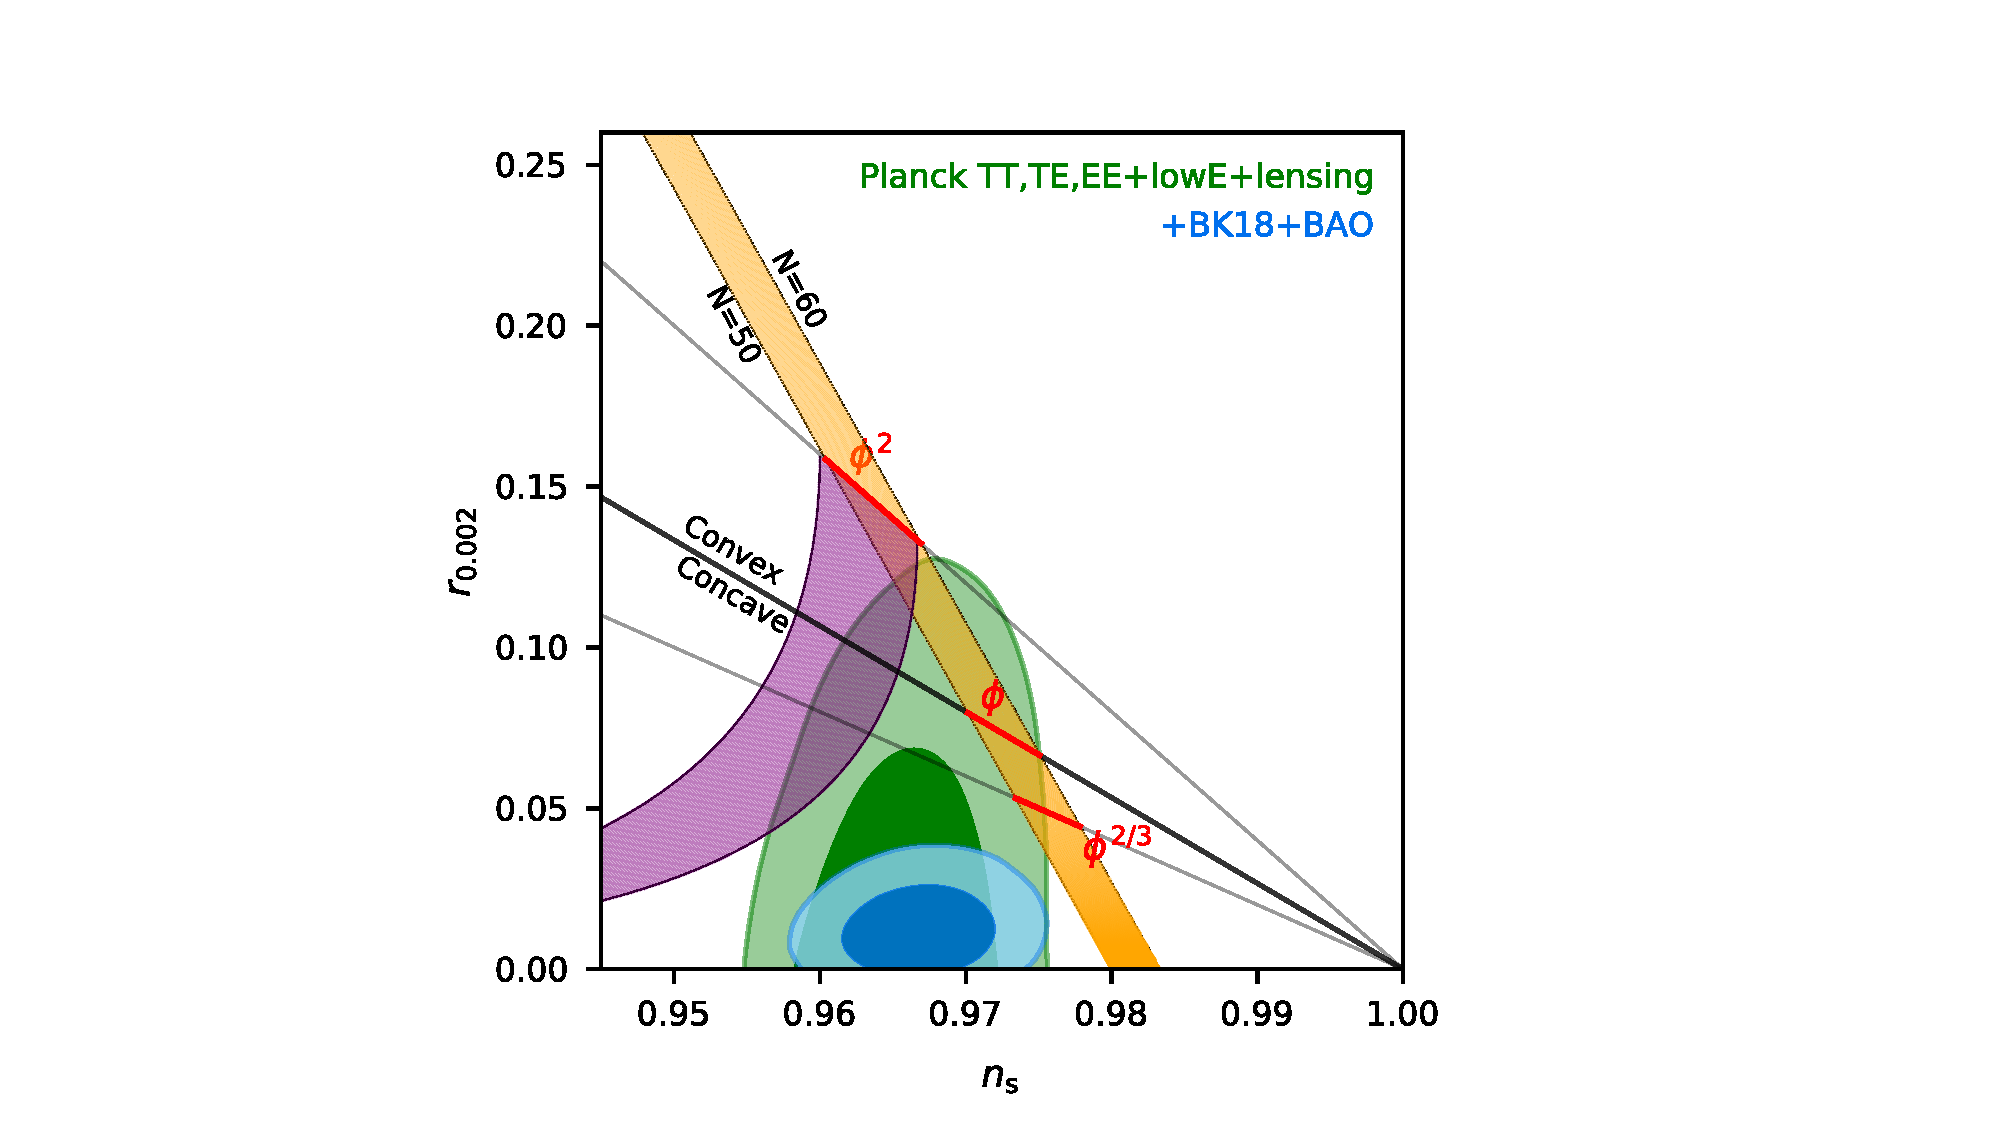
\includegraphics[width=140mm,height=85mm]{Sections/Figures/SpectralIndex.pdf} 
\caption{The most recent constraints on inflationary models in the tensor-to-scalar ratio $r$ and spectral index $n_s$ plane, taken from \cite{BICEP:2021xfz}. A substantial amount of inflationary models are already in tension with observations. } \label{Fig:SpectralIndex} 
\end{center}
\end{figure}



\subsection{Multi-field Inflation}
\label{sec:multinf}

So far, we have discussed the simplest (vanilla) inflationary scenario, where a single canonically normalised scalar field drives inflation. However, as discussed at more length in Sec. \ref{ModuliSection}, in string theory there are usually many scalar fields (as well as other fields of various spin) which may either drive inflation or act as spectator fields with interesting cosmological implications. In what follows, we briefly review these possibilities from a pure field theory perspective, which will be important for our discussion on string inflation in Sec. \ref{sec:infla}.

Let us consider the  Lagrangian for several scalar fields, minimally coupled to gravity\footnote{For a recent review on multi-field inflation in field theory see \cite{Gong:2016qmq}.}:
\be\label{4Daction}
S= \int{d^4x \sqrt{-\tt g} \left[\Mp^2 \frac{R}{2}  - \frac12\,g_{ab}(\phi^c) \partial_\mu\phi^a \partial^\mu\phi^b - V(\phi^a)\right]} \,,
\ee
where $g_{ab}$ is the {\em field space metric}.  The equations of motion derived from this action are given by
\bea
&&H^2 = \frac{1}{3\Mp^2} \left(\frac{\dot \varphi^2}{2}  + V(\phi^a)\right) \,, \label{H} \\
&& \ddot \phi^a + 3H\dot\phi^a + \Gamma^a_{bc} \dot\phi^b\dot\phi^c + g^{ab} V_{,b} =0  \,,
\label{phis}
\eea
where
\be\label{varphi}
\dot\varphi^2 \equiv g_{ab} \dot \phi^a\dot\phi^b\,
\ee
and the Christoffel symbols in \eqref{phis} are computed using the scalar manifold metric $g_{ab}$, while $V_{,a}$ denotes derivatives with respect to the scalar field $\phi^a$.



The slow-roll conditions and rapid turning in multi-field inflation  can be understood neatly  using a  kinematic basis to decompose the inflationary trajectory into {\em tangent} and {\em normal} directions  (i.e.~adiabatic and entropic). Focusing on the two field case for concreteness, we introduce   unit tangent (adiabatic) and normal (entropic) vectors  $T^a$ and $N^a$, as follows:
\be
T^a = \frac{\dot\phi^a}{\dot\varphi}\,, \qquad T^aT_a =1\,,\qquad
N^aT_a=0, \qquad N^aN_a=1\,.
\ee
The  equations of motion \eqref{phis} for the scalars $\phi^a$ projected along these two directions become:
\bea
 \ddot\varphi + 3H\dot\varphi + V_T & = &0 \,, \label{varphiT}\\
D_t T^a  + \Omega N^a &=&0\,,\label{varphiN}
\eea
 where $V_T = V_{,a}T^a$, $V_N = V_{,a}N^a$ and the {\em turning rate} parameter, $\Omega$, is defined as
\be\label{Omega}
\setlength\fboxsep{0.25cm}
\setlength\fboxrule{0.4pt}
\boxed{
\Omega \equiv \frac{V_N}{\dot\varphi}\,.}
\ee
The field-space covariant time derivative is  defined as:
 \be\label{Dt}
 D_tT^a \equiv \dot T^a + \Gamma^{a}_{bc} T^b \dot \phi^c \,.
 \ee

Using the equations of motion, we can  write  the projections of the Hessian elements along the tangent vector as  \cite{Achucarro:2010da,Hetz:2016ics,Christodoulidis:2018qdw,Chakraborty:2019dfh}:
\be\label{VTT1}
\frac{V_{TT}}{3H^2} =  \frac{\Omega^2}{3H^2} + 2\,\epsilon -\frac{\eta}{2} -
\frac{\xi_\varphi}{3}   \,,
\ee
as well as the projection along $T $ and $N$ as \cite{Aragam:2021scu}:
\be
\label{VTN1}
\frac{V_{TN}}{3H^2} = w\left( 1-\epsilon+\frac\eta3+\frac\nu3 \right).
\ee
In these equations  we  introduced  the slow-roll parameter
\be
\xi_\varphi\equiv \frac{\dddot\varphi}{H^2 \dot\varphi}\,,
\ee
as well as the {\em dimensionless turning rate}, $w$, which measures the {\em non-geodesicity} of the trajectory:
\be\label{eq:w}
\setlength\fboxsep{0.25cm}
\setlength\fboxrule{0.4pt}
\boxed{
w \equiv \frac{\Omega}{H}\,,}
\ee
and a new {\em slow-roll} parameter, which arises only in the multi-field case, $\nu$:
\be\label{eq:nu}
\setlength\fboxsep{0.25cm}
\setlength\fboxrule{0.4pt}
\boxed{
\nu\equiv \frac{\dot w}{H\,w}\,.}
\ee

\smallskip

\ni Note  that the expressions \eqref{VTT1}, \eqref{VTN1}  {\em are exact}, as we have not made use of any slow-roll approximations.
 On the other hand, $V_{NN}$ depends on the inflationary trajectory in a model-dependent fashion.

\subsubsection{Slow-roll in multi-field inflation}

Let us revisit the slow-roll conditions in the case that more than one field is present. These  require the  slow-roll parameters $\epsilon, \eta, \delta_\varphi $ above, to be much smaller than one in order to guarantee long-lasting, slow-roll inflation, that is,  $\epsilon, \eta, \delta_\varphi, \xi_\varphi \ll 1$. It is easy to check that these conditions imply
\bea
&&H^2 \simeq \frac{V}{3M_{Pl}} \,, \\
&& 3 H\dot \varphi + V_T \simeq 0 \,, 
\eea
and thus that the tangent projection of the derivative of the potential needs to be  small:
\be\label{epT}
\epsilon_T \equiv \frac{M_{Pl}^2}{2} \left(\frac{V_T}{V}\right)^2 \ll1  \,.
\ee
On the other hand, the normal projection $V_N$ can be large,  and it is related to the turning rate defined in eq.~\eqref{Omega}.
Moreover, from \eqref{VTT1} we see that during slow-roll, the equations of motion imply
\be\label{VTTsr}
\frac{V_{TT }}{3H^2} \sim \frac{\Omega^2}{3H^2}\,,
\ee
while from \eqref{VTN1}, requiring $\eta\ll1$ (equivalently $\delta_\varphi \ll 1$) implies that (barring possible cancellations)
\be\label{VTN_slowroll}
   \frac{V_{TN}}{3H^2}\sim \frac{ \Omega}{H} \,, \qquad {\rm and} \qquad
     \nu \ll 1\,.
\ee
Hence, we see that $\nu$ behaves as a new slow-roll parameter in multi-field inflation: the turning rate is guaranteed to be slowly varying during slow-roll \cite{Aragam:2020uqi,Aragam:2021scu}.

We see then that in the multi-field case, slow-roll inflation does not require small eigenvalues of the Hessian \cite{Chakraborty:2019dfh,Aragam:2021scu}, as usually believed. Namely, defining the multi-field generalisation of the $\eta_V$ parameter \eqref{eq:etaV} as
\be\label{etaVmulti}
\setlength\fboxsep{0.25cm}
\setlength\fboxrule{0.4pt}
\boxed{
\eta_V^{ m} \equiv \Mp^2 \left|{\rm min\,\,\, eigenvalue}  \left(\frac{ \nabla^a \nabla_b V}{V}\right)\right|, }
\ee
it is clear that $\eta_V^m$ does not need to be small and indeed can  be much  larger than one in multi-field inflation \cite{Chakraborty:2019dfh,Aragam:2021scu}. This implies that in multi-field inflation, all inflatons can be heavier than the Hubble scale \cite{Chakraborty:2019dfh}.
Thus the $\eta$-problem in multi-field inflation may manifest itself, if present, in a different form. For example, the curvature of the field space metric, $R_{\rm fs}$, may in general be non-zero and in particular could be large (in Planck units). Therefore, this introduces a new scale, and the flatness of the potential may be constrained over this new scale (see e.g.~\cite{Renaux-Petel:2021yxh}). However, in general, we expect $R_{\rm fs}$ to be of order one in Planck units.

\subsubsection*{ Multi-field inflation and swampland constraints}

Let us finally make some comments  between multi-field  inflation and the recently proposed dS conjectures \cite{Obied:2018sgi,Garg:2018reu,Ooguri:2018wrx}, which require that (see Section \ref{Sec:Swamp})
\bea\label{eq:swamp1}
 \frac{\nabla V}{V} \geq \frac{c}{\Mp}  \qquad {\text{or}}  \qquad %\\
  \frac{{\rm min} (\nabla^a \nabla_b V)}{V} \leq -\frac{c'}{\Mp^2},
\eea
where $c, c'$ are  ${\cal O}(1)$ constants.
From our discussion on  slow-roll inflation in the multi-field case, it can be easily seen that  the first condition in \eqref{eq:swamp1} can be satisfied, so long as the  turning rate $\Omega/H$  is sufficiently large \cite{Achucarro:2018vey}.
Indeed, the potential slow-roll parameter \eqref{eq:epsV} in  the multi-field case is given by
\be\label{epsimulti}
\epsilon_V^m \equiv \frac{\Mp^2}{2} \frac{V^aV_a}{V^2} = \epsilon_T + \frac{\Omega^2}{9H^2}\epsilon \,.
\ee
For $\epsilon_T\simeq \epsilon$,  one arrives at the relation  \cite{Achucarro:2018vey,Hetz:2016ics}:
\be\label{epsV2}
\epsilon_V^m \simeq \epsilon\left(1  + \frac{\Omega^2}{9H^2}\right)\,,
\ee
and therefore we see that in a multi-field inflationary model, where $\Omega\ne 0$, for sufficiently large turning rate  $\Omega/H$  $\epsilon_V^m$ can be comparable to or larger than one.
On the other hand, the second condition in \eqref{eq:swamp1} is precisely the requirement that $\eta_V^m$  be large (with negative eigenvalue). As we discussed above, this can happen in mulltifield slow-roll inflation without disrupting it\footnote{A field theory example with large values of $c'$ is given in \cite{Christodoulidis:2018qdw}. Supergravity examples with large $c'$ are given in \cite{Aragam:2021scu}.}.
In summary, multi-field inflation allows for  new inflationary attractors, which do not need to satisfy the single field potential flatness conditions \eqref{eq:epsV}, \eqref{eq:etaV}.



\subsubsection{Cosmological perturbations, the multi-field case}

The presence of more than one field changes the kinds of primordial fluctuations which are possible, because with several fields there can be perturbations,  for which the total energy density, $\delta\rho=0$, remains unchanged. Such fluctuations are called  {\em isocurvature} fluctuations, in contrast to the {\em adiabatic} fluctuations involving nonzero $\delta\rho$ considered in the single field case.

There are strong observational constraints on the existence of isocurvature fluctuations and current observations are consistent with purely adiabatic oscillations at horizon re-entry  \cite{Planck:2018vyg,Planck:2018jri}. Primordial isocurvature modes need not be a problem for an inflationary model even if they are generated at horizon exit, provided they are subsequently erased before horizon re-entry. Moreover, the presence of more than one field can give rise to large non-Gaussianties in the power spectrum, which are also constrained by observations \cite{Planck:2019kim}. At the same time, additional scalars -- as well as other higher spin fields -- may give rise to interesting phenomenology and are thus of great interest for future 
%
experiments\footnote{See \cite{Arkani-Hamed:2015bza,Lee:2016vti,Alexander:2019vtb} for studies  of the imprints of new (higher spin) particles on the non-gaussianities of the cosmological fluctuations and \cite{Alexander:2020gmv,Criado:2020jkp,Jenks:2022wtj,Gondolo:2021fqo} for proposals of dark matter as higher spin fields, and their phenomenology.
}.

\subsubsection{Spectator fields during inflation}

Scalar fields acting as spectators during inflation are well motivated not only from a purely field theory perspective, but also from a phenomenological point of view. Any additional fields may give rise to interesting features that could produce observable effects which would then be of great importance. The same can be said for spin one fields such as $U(1)$ vector fields, producing for example   anisotropies, as well as $SU(2)$ gauge fields, potentially sourcing  tensor perturbations, and evading the Lyth bound discussed above (see e.g.~\cite{Maleknejad:2012fw} for a review).
We will not review here the vast literature on the subject, but will mention some interesting possibilities in the context of string cosmology in Sec. \ref{sec:infla}.

\subsection{Quintessence}\label{sec:quint}

As we mentioned before (see Sec.~\ref{subsecME}),  current observations provide strong evidence for the current acceleration of the universe.
In the $\Lambda$CDM standard model of cosmology, this is due to a constant vacuum energy, $\Lambda$.
However, the constant vacuum energy appears to be  much smaller than  would be expected from estimates based on quantum field theory. This has led to the  widespread speculation that the vacuum energy may not be constant, but it may now be small because the universe is old. Such a  time-varying vacuum energy is called {\em quintessence} \cite{Wetterich:1987fm,Peebles:1987ek,Ratra:1987rm}.\footnote{The name quintessence was coined in \cite{Caldwell:1997ii}. For reviews and several references see e.g.~\cite{Copeland:2006wr,Linder:2007wa,Tsujikawa:2013fta}.}

The natural way to introduce a time-varying vacuum energy is to assume the existence of one or more scalar fields, on which the vacuum energy depends, and whose cosmic expectation values change with time. We have seen that scalar fields of this type  play a crucial role in cosmological inflation and thus the discussion of quintessence uses several of the concepts which already appear in inflation.
Considering a single scalar field, the idea is that its dynamics drive the present epoch of accelerated expansion. Dark energy started to dominate relatively recently, namely less than a single e-fold ago (see Fig.~\ref{fig:RhoEvol}). It may therefore seem easy to have a sufficiently flat scalar potential, which starts dominating the energy density less than an e-folding ago.
The original and simplest example is provided by the following potential \cite{Wetterich:1987fm,Peebles:1987ek,Ratra:1987rm}
\be
\label{eq:QV}
V(\phi) = M^{4+\alpha} \phi^{-\alpha},
\ee
where $\alpha$ is positive but otherwise arbitrary, and $M$ is a constant with units of mass. We can call this type of potential  {\em runaway} like. We give a brief discussion here, but explore this class of runaway potentials in string theory more in Sec. \ref{reheating} and Sec. \ref{sec:DE}, in the context of both transient post-inflationary runaways and also quintessence dynamics in the late-time universe. 
The model \eqref{eq:QV} can be solved in some detail as a concrete example of quintessence (see e.g.~\cite{Weinberg:2008zzc} and further discussion in Sec. \ref{sec:DE}).

Any successful quintessence must have the property that at early times, the energy density of the quintessence field is subdominant over radiation to avoid conflict with BBN. With potential \eqref{eq:QV}, one can show that the field has a solution at early times during radiation domination such that
\be
\rho_\phi\propto t^{-2\alpha/(\alpha+2)}\,,
\ee
and thus at early times ($t\ll 1$) $\rho_\phi$ is indeed less than $\rho_r$ which goes as $t^{-2}$. This solution turns out 
to be an attractor, known as a {\em tracker solution}. After radiation domination, the universe undergoes an epoch of matter domination, but the tracker solution of $\phi$ continues to have energy density falling as $\rho_\phi\sim t^{-2\alpha/(\alpha+2)}$, and since $\rho_r$ and $\rho_m$ decrease faster ($t^{-8/3}, t^{-2}$ respectively in matter domination) eventually, both will fall below $\rho_\phi$. 

At late times, 
one finds $\rho_\phi\propto t^{-\alpha/(2+\alpha/2)}$, or $\ln a \propto t^{2/(2+\alpha/2)}$ and the expansion is  dominated by the quintessence field.  The point when $\rho_m=\rho_\phi$ is given by
$t_c\approx M^{-(4+\alpha)/2}G_4^{-(2+\alpha)/4}$, which gives $\phi(t_c)\approx G_4^{-1/2}$. 
Finally, to achieve agreement with observations, setting the critical time $t_c$ at which $\rho_m\approx \rho_\phi$ to be close to the present moment $t_0 \approx 1/H_0$,  requires the constant factor in $V(\phi)$ to take the value
\be
M^{4+\alpha} \approx G_4^{-1-\alpha/2}H_0^2\,.
\ee
There is, however, no fundamental explanation as to why this should be the case.

Although quintessence has been proposed as a potential candidate to explain the current acceleration, it still faces several challenges. We will discuss later on  in more detail how these manifest  in the context of string theory (see Sec.~\ref{sec:ChallengesQ}), but let us briefly mention here some of the main challenges for any model of quintessence.
\bi
 \item {\em Fine-tunings}. As can be evident from the above discussion, quintessence models need to explain why the field has to be exactly at the point where $V(\phi_0) \simeq \rho_0 \simeq (0.003 \,{\rm eV})^4$ today. Moreover, it is not hard to check that a successful quintessence model requires the mass of the field to be extremely light, $m_\phi\simeq H_0\simeq 10^{-33}\,{\rm eV}$ (at least in the case of single field), which must be protected against quantum corrections.

\item {\em Phenomenological constraints}. Phenomenological problems to realise quintessence arise as the quintessence field must be extremely weakly coupled to ordinary matter;  otherwise, its exchange would generate observable long-range forces, which are severely constrained by experiments.
The quintessence field can be a scalar as we saw above, or a pseudoscalar, such as an axion.\footnote{Other fields have also been proposed as quintessence, however the same problems arise as for the scalar case.} The advantage of axions is that they can avoid  fifth-force constraints, but a typical axion potential requires a trans-Planckian decay constant to drive any successful period of accelerated expansion.
\ei


\subsection{Possible Tensions with $\Lambda$CDM?}

We end this overview section on cosmology with mention of various possible hints towards tensions between Planck observations of the CMB and other cosmological probes.  Although the statistical significance of these tensions is not definitive, and even still under debate, if any are confirmed and not due to systematics, this would be exciting evidence of new physics beyond the $\Lambda$CDM model.  

The most famous of these tensions is the Hubble tension.  Planck constraints on today's Hubble parameter, which is obtained by assuming the standard six parameter $\Lambda$CDM model, yields $H_0 = 67.44 \pm 0.58 {\rm km}\,{\rm s}^{-1}\,{\rm Mpc}^{-1}$ \cite{Planck:2018vyg}.  This is to be contrasted with recent direct local distance ladder measurements of $H_0$ from the SH0ES collaboration, which gives instead $H_0 = 74.03 \pm 1.42 {\rm km}\,{\rm s}^{-1}\,{\rm Mpc}^{-1}$ \cite{Riess:2019cxk}. This amounts to a $4.3\sigma$ discrepancy, with other direct measurements going in the same direction.  For a recent review on the $H_0$ discrepancies and phenomenological solutions see \cite{DiValentino:2021izs}; see \cite{Efstathiou:2020wxn} for a critical perspective. Proposals to resolve the tension include increasing the number of effective neutrino species $N_{\rm eff}$, modifying the dark energy equation of state, and the presence of some early dark energy; for a systematic comparison of several proposals and their relative success see \cite{Schoneberg:2021qvd}.  A review of all the current discordances, covering $H_0$, the $\sigma_8$--$S_8$ tension, and other less statistically significant anomalies, together with an experimental outlook, is given in \cite{Abdalla:2022yfr}.

\enddocument


\newpage
